% (C) Marc Lijour, 2021 
% Licensed under a Creative Commons License BY-SA
% https://creativecommons.org/licenses/by-sa/2.5/ca/
% Introduction to blockchain
% Hands-on Introduction
% Presentation touching upon:
% - What is blockchain
% - Hand-on introduction to “crypto” (digital currency, tokens, wallets)
%
% Chrome persona: Workshop July

\frame{
	\frametitle{Who am I?}
	\framesubtitle{\url{https://www.linkedin.com/in/marclijour/}}
	\begin{columns}
	\column{0.3\textwidth}
		\begin{figure}
		
\includegraphics[width=2cm]{../pics/logos/colliderx_logo}
		\end{figure}
	\column{0.3\textwidth}
		\begin{figure}
		
\includegraphics[width=3.5cm]{../pics/logos/consensys-logo-v-630x581}
		\end{figure}
	\column{0.3\textwidth}
		\begin{figure}
		
\includegraphics[width=3cm]{../../Metamesh-LaTeX_Templates/images/logo-black}
		\end{figure}

		\begin{figure}
		
\includegraphics[width=3cm]{../../Creative_Emergy-LaTeX_Templates/images/ce_logo_hr_name}
		\end{figure}
	\end{columns}
}

%\frame{ 
%	\frametitle{Access these slides}
%	\center\Huge 
%	\url{https://bit.ly/2lJbAnB}\\ 
%	\vspace{2em}
%	{\normalsize 
%		or find in the folder \href{https://bit.ly/2k95zQW}{GBC - Blockchain Developer Certificate} at\\
%		\url{https://github.com/marclijour/presentations}
%	}
%}

% ======================================================================================================
%                         Introduction to the presentation and What is Blockchain 
% ======================================================================================================
\section{What is Blockchain?}
\frame{
	\frametitle{The Trust Machine}
	\begin{figure}
		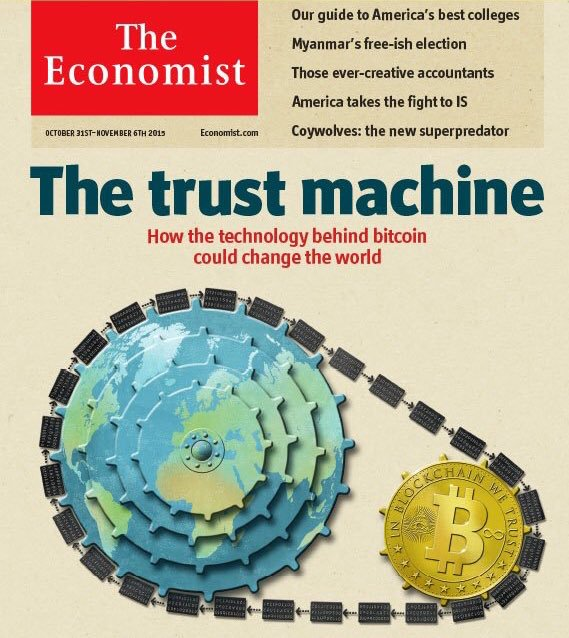
\includegraphics[height=6cm]{../pics/blockchain/economist-trust-machine}
	\end{figure}
}

\frame{
	\frametitle{Source of Trust}
	\framesubtitle{\href{https://www.youtube.com/watch?v=6WG7D47tGb0}{World Economic Forum: \textit{What is Blockchain} Youtube Video}}
	\begin{figure}
		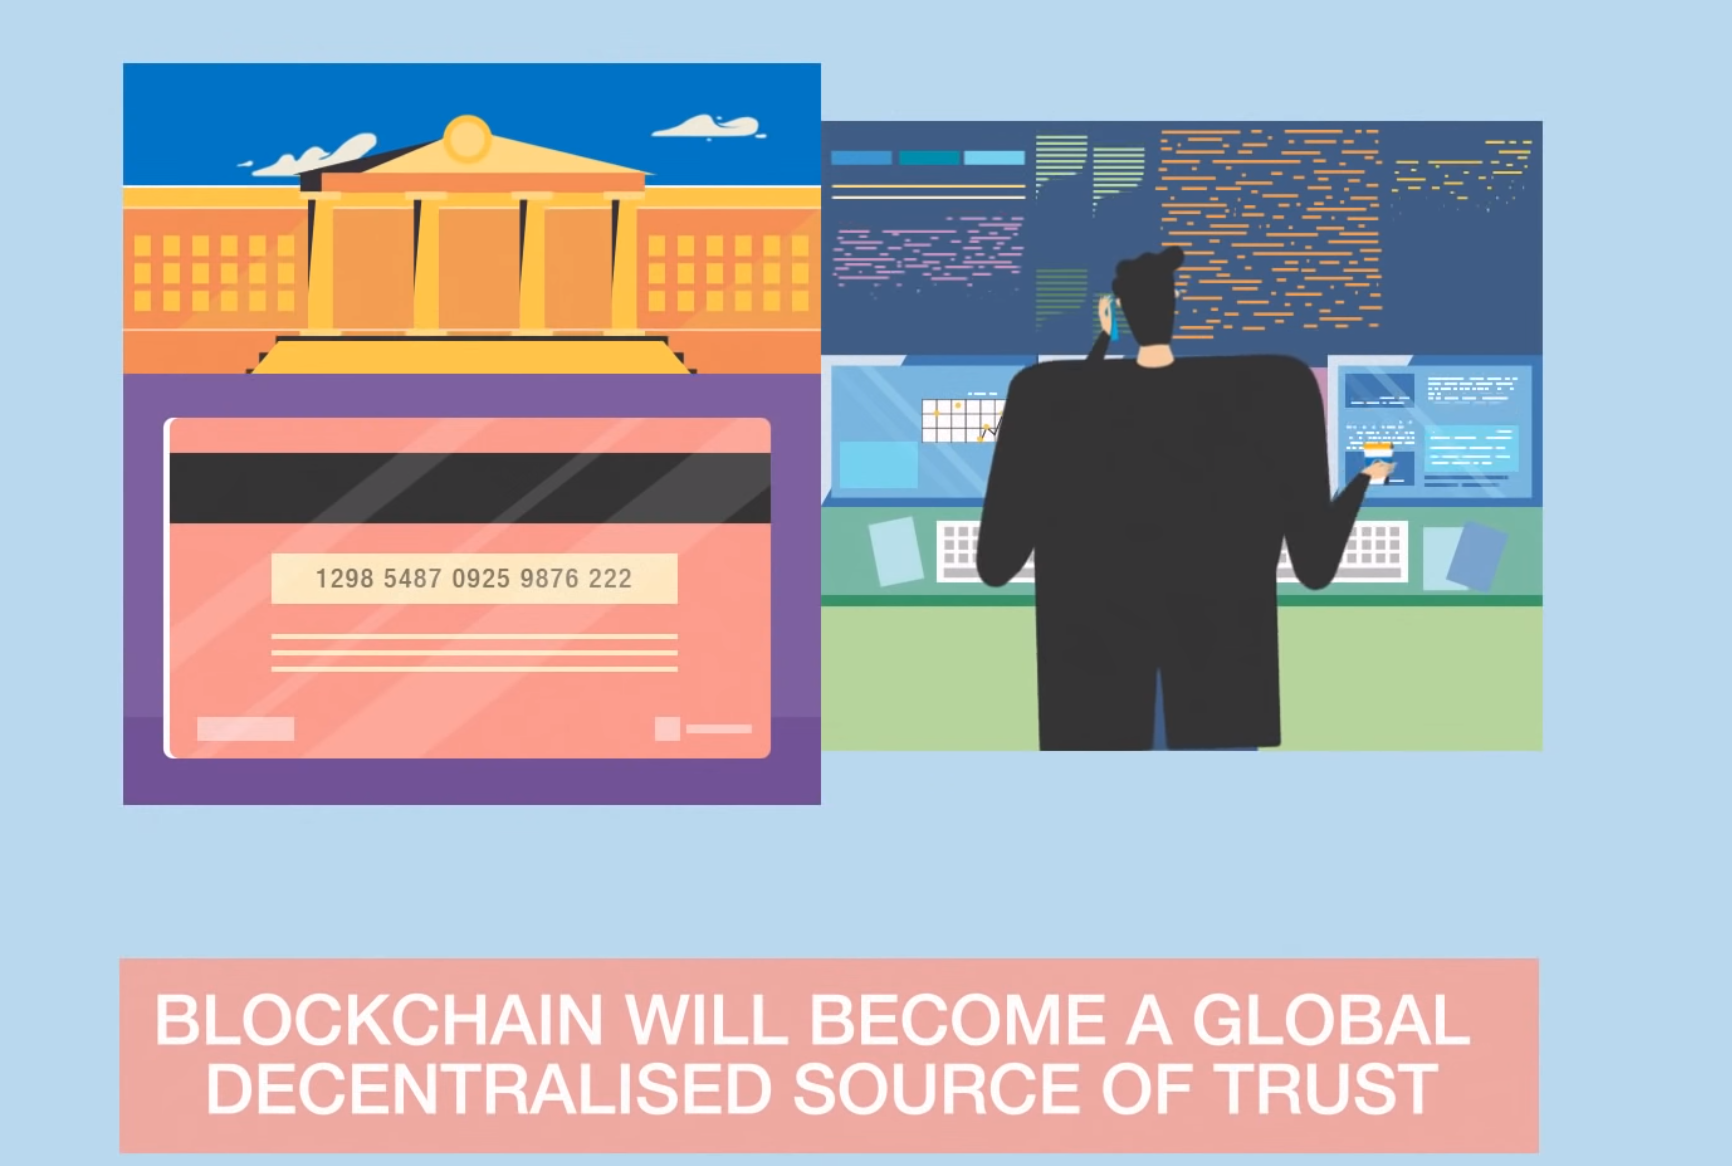
\includegraphics[width=11cm]{../pics/blockchain/wef-blockchain-source-of-trust}
	\end{figure}
}

\frame{
	\frametitle{Key Cryptographic Primitives}
	\begin{columns}[T]
	\column{0.3\textwidth}
		\centering \textbf{Signing}
		\begin{figure}
		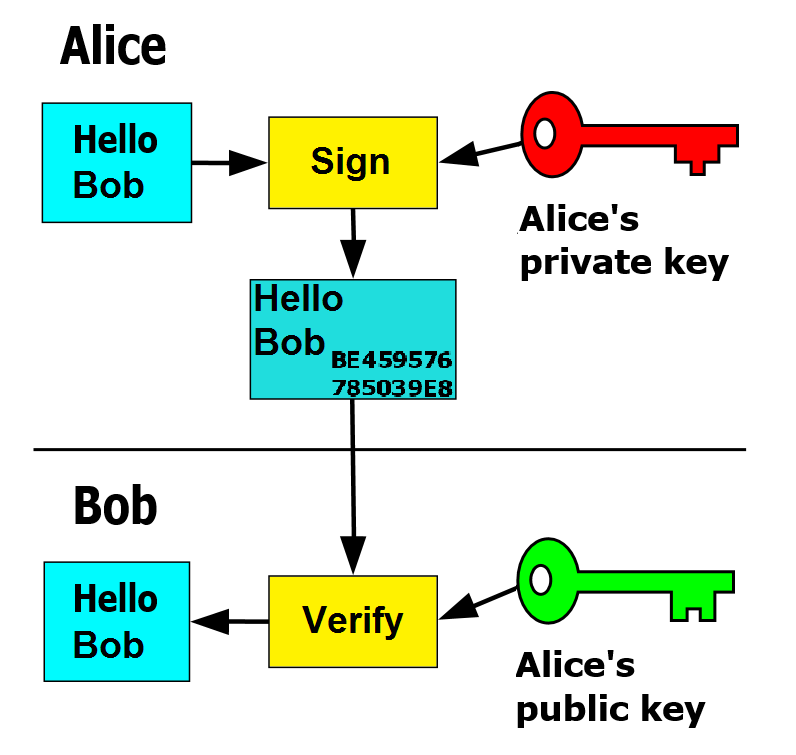
\includegraphics[width=3cm]{../pics/cryptography/Private_key_signing}
		\\
		% CC-BY-SA
		\tiny{Credit: \href{https://commons.wikimedia.org/wiki/User:FlippyFlink}{FlippyFlink}}
		\end{figure}
	\column{0.3\textwidth}
		\centering \textbf{Encrypting}
		\begin{figure}
		% https://en.wikipedia.org/wiki/File:Public_key_encryption.svg
		% public domain
		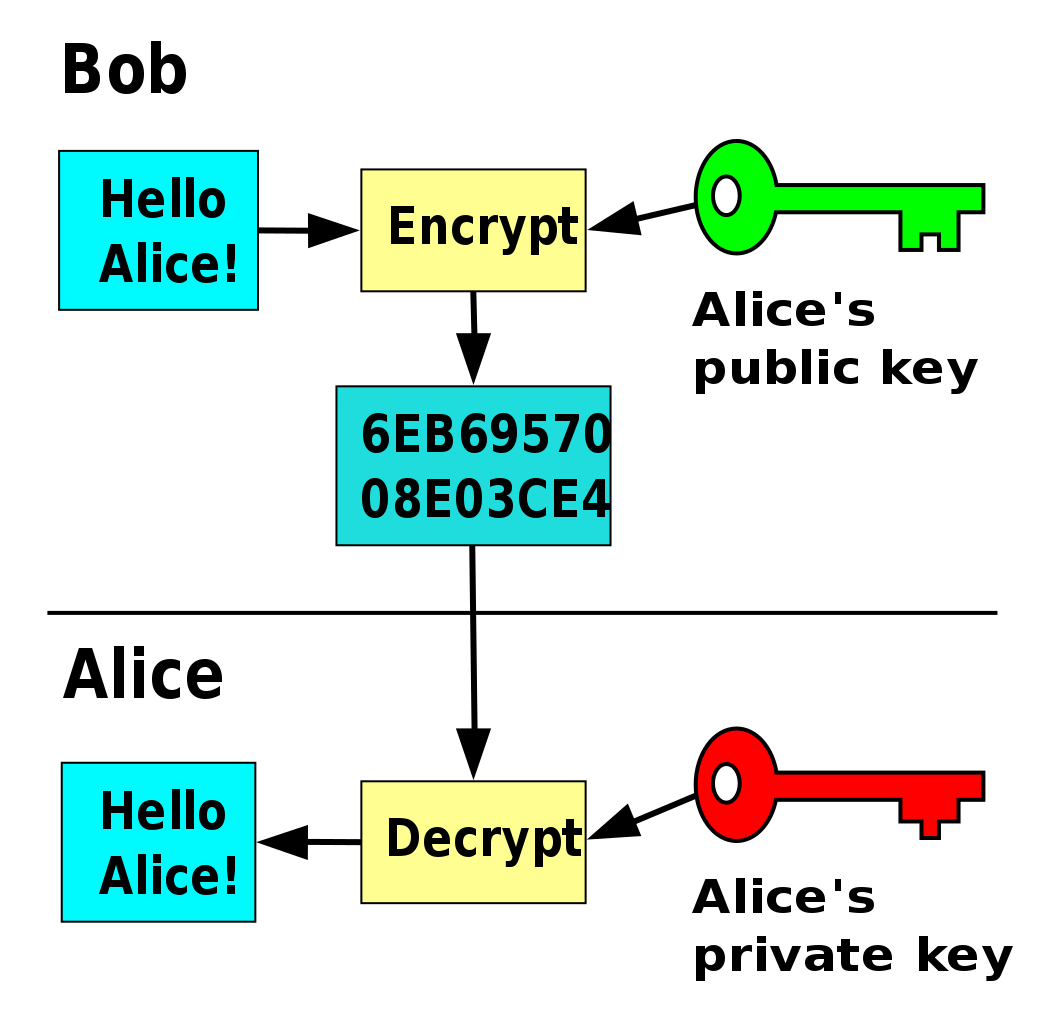
\includegraphics[width=3cm]{../pics/cryptography/1050px-Public_key_encryption}
		\end{figure}
	\column{0.3\textwidth}
		\centering \textbf{Hashing}
		\begin{figure}
		% https://commons.wikimedia.org/wiki/File:Cryptographic_Hash_Function.svg
		% public domain
		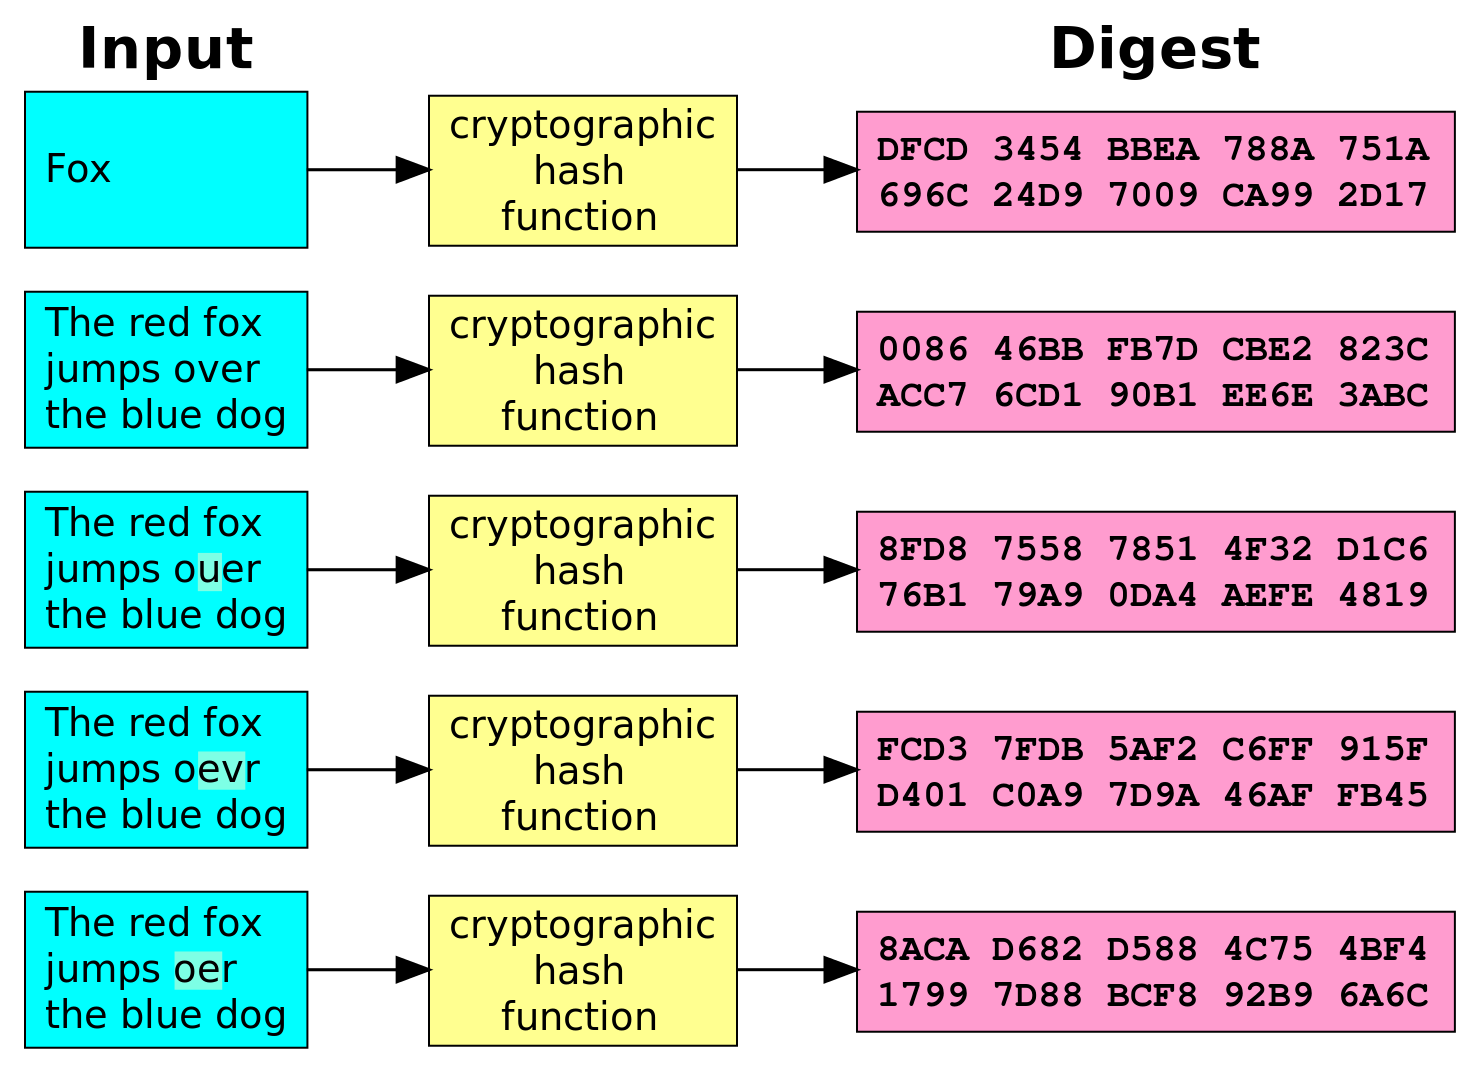
\includegraphics[width=3.6cm]{../pics/cryptography/Cryptographic_Hash_Function}
		\end{figure}
	\end{columns}
}

\frame{
	\frametitle{Where do we need more trust?}
	\begin{itemize}
		\item payments
		\pause
		\item national identity
		\pause
		\item supply chain (e.g. food: \href{https://www.ctvnews.ca/business/france-holds-trial-over-horse-meat-used-in-school-lunches-frozen-lasagna-1.4261868}{Spanghero horse meat trial}, Opioids, expensive cargos)
		\pause
		\item contracts 
		\pause
		\item \textit{real} news \& historical events (e.g. \href{https://media.consensys.net/holding-war-criminals-accountable-with-the-ethereum-blockchain-6b12471a7cdd}{bombings})
		\pause
		\item collaborative data reporting
		\item \ldots
	\end{itemize}
}

% ======================================================================================================
%                         Hands-on Introduction to Crypto, Wallets, and Custom Tokens 
% ======================================================================================================
\section{Hands-on Introduction to Crypto}
\frame{
	\frametitle{}
	\centering\Huge
	Let's try things out!
}

\frame{
	\frametitle{Install MetaMask}
	\begin{columns}
	\column{0.6\textwidth}
		Follow step by step:
		\begin{enumerate}
			\item Install the \href{https://chrome.google.com/webstore/detail/metamask/nkbihfbeogaeaoehlefnkodbefgpgknn}{Chrome/Chromium extension} 
			\item Watch the \href{https://www.youtube.com/watch?v=6Gf\_kRE4MJU}{intro on Youtube}
			\item Create an account 
			\item Switch to the Ropsten Testnet (top-right in MetaMask) 
			\item Fill your account with Ether from \url{https://faucet.metamask.io}
		\end{enumerate}
	\column{0.4\textwidth}
		\begin{figure}
			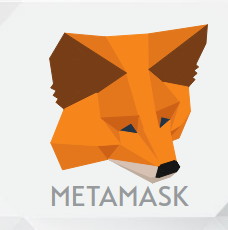
\includegraphics[width=3cm]{../pics/ethereum/metamask-logo}
			\captionsetup{justification=centering}
			\caption*{\url{https://metamask.io}}
		\end{figure}
	\end{columns}
}

\frame{
	\frametitle{Create a new Wallet}
	\begin{figure}
		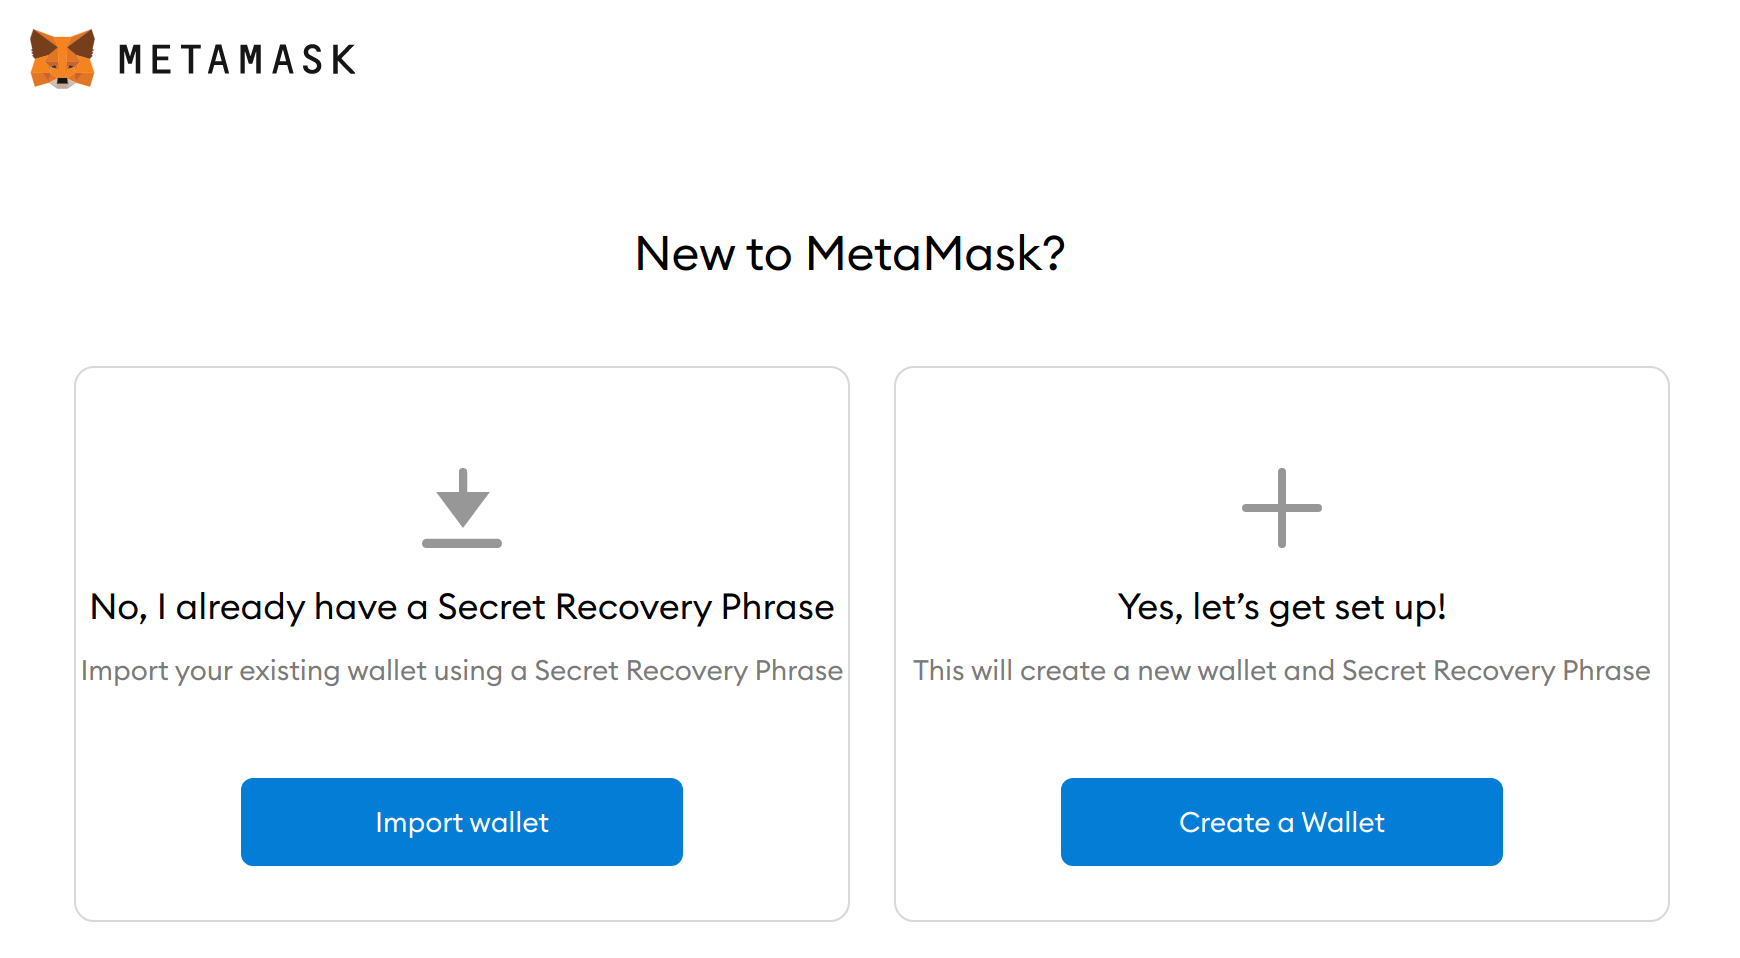
\includegraphics[width=11cm]{../pics/ethereum/metamask-first-step}
	\end{figure}
}

\frame{
	\frametitle{Discover your secret backup phrase}
  \framesubtitle{aka seed phrase, aka the 12 words}
	\begin{figure}
		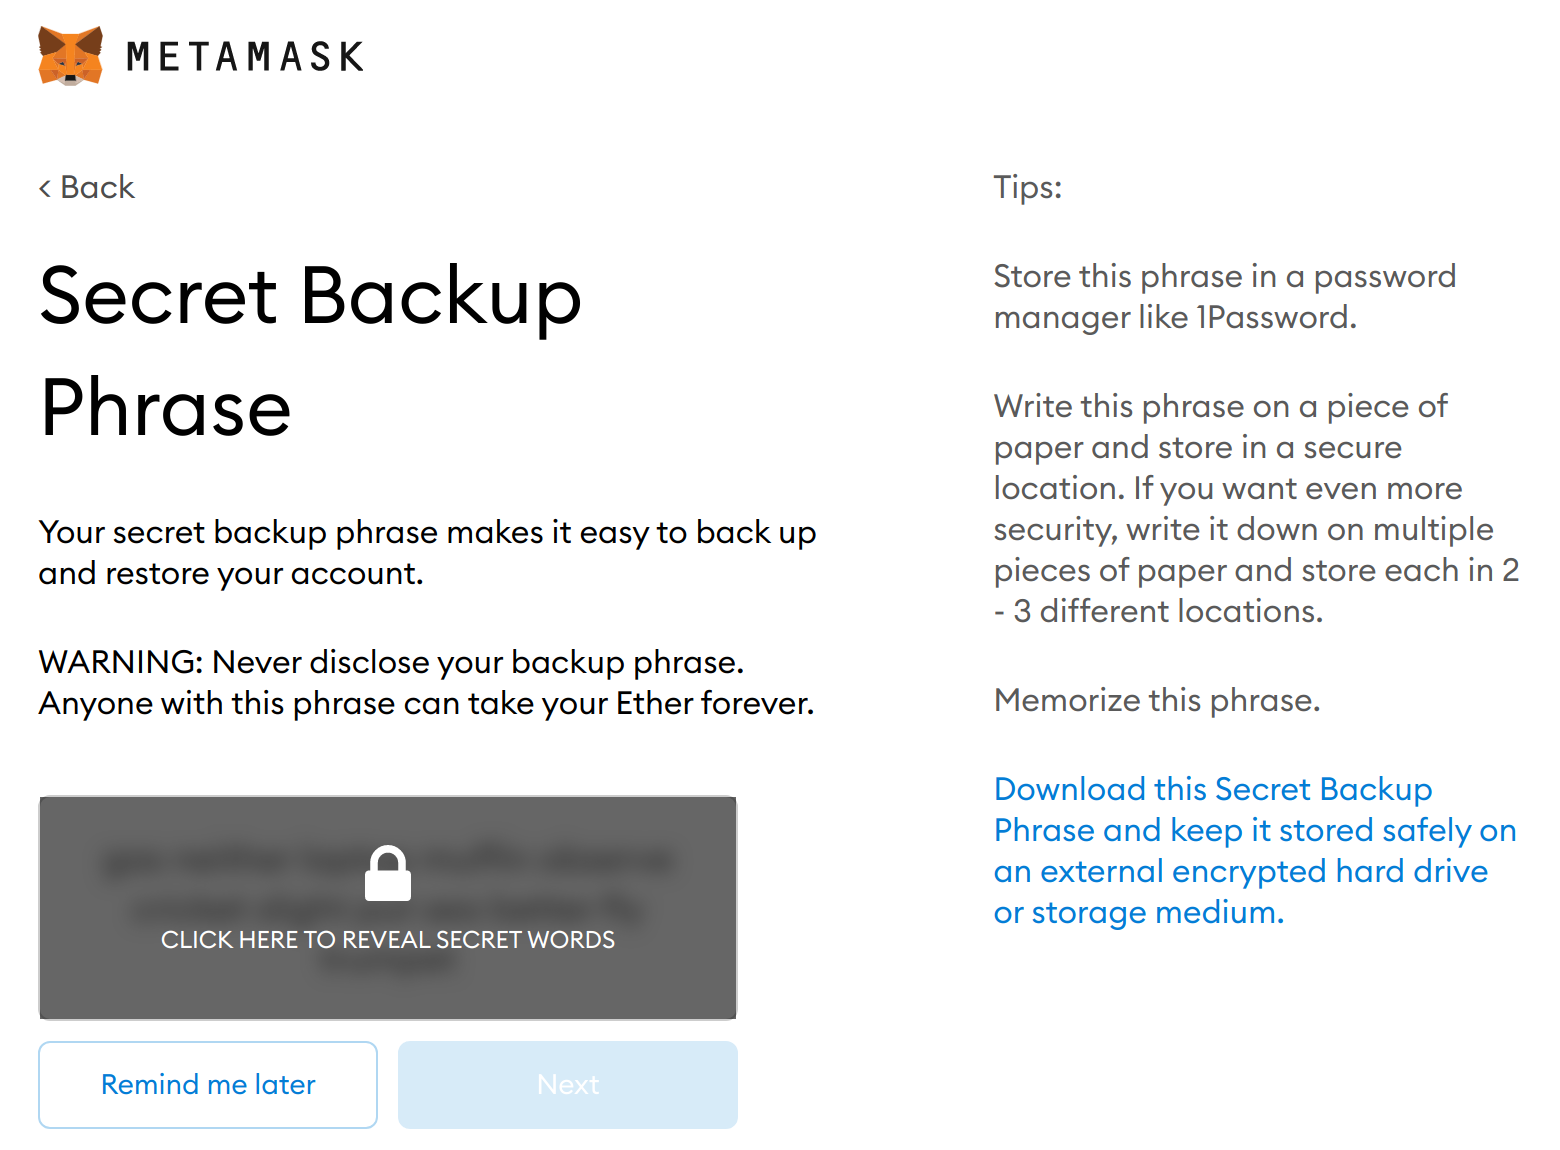
\includegraphics[width=10cm]{../pics/ethereum/metamask-backup-phrase}
	\end{figure}
}

\frame{
	\frametitle{Fully setup Wallet}
	\begin{figure}
		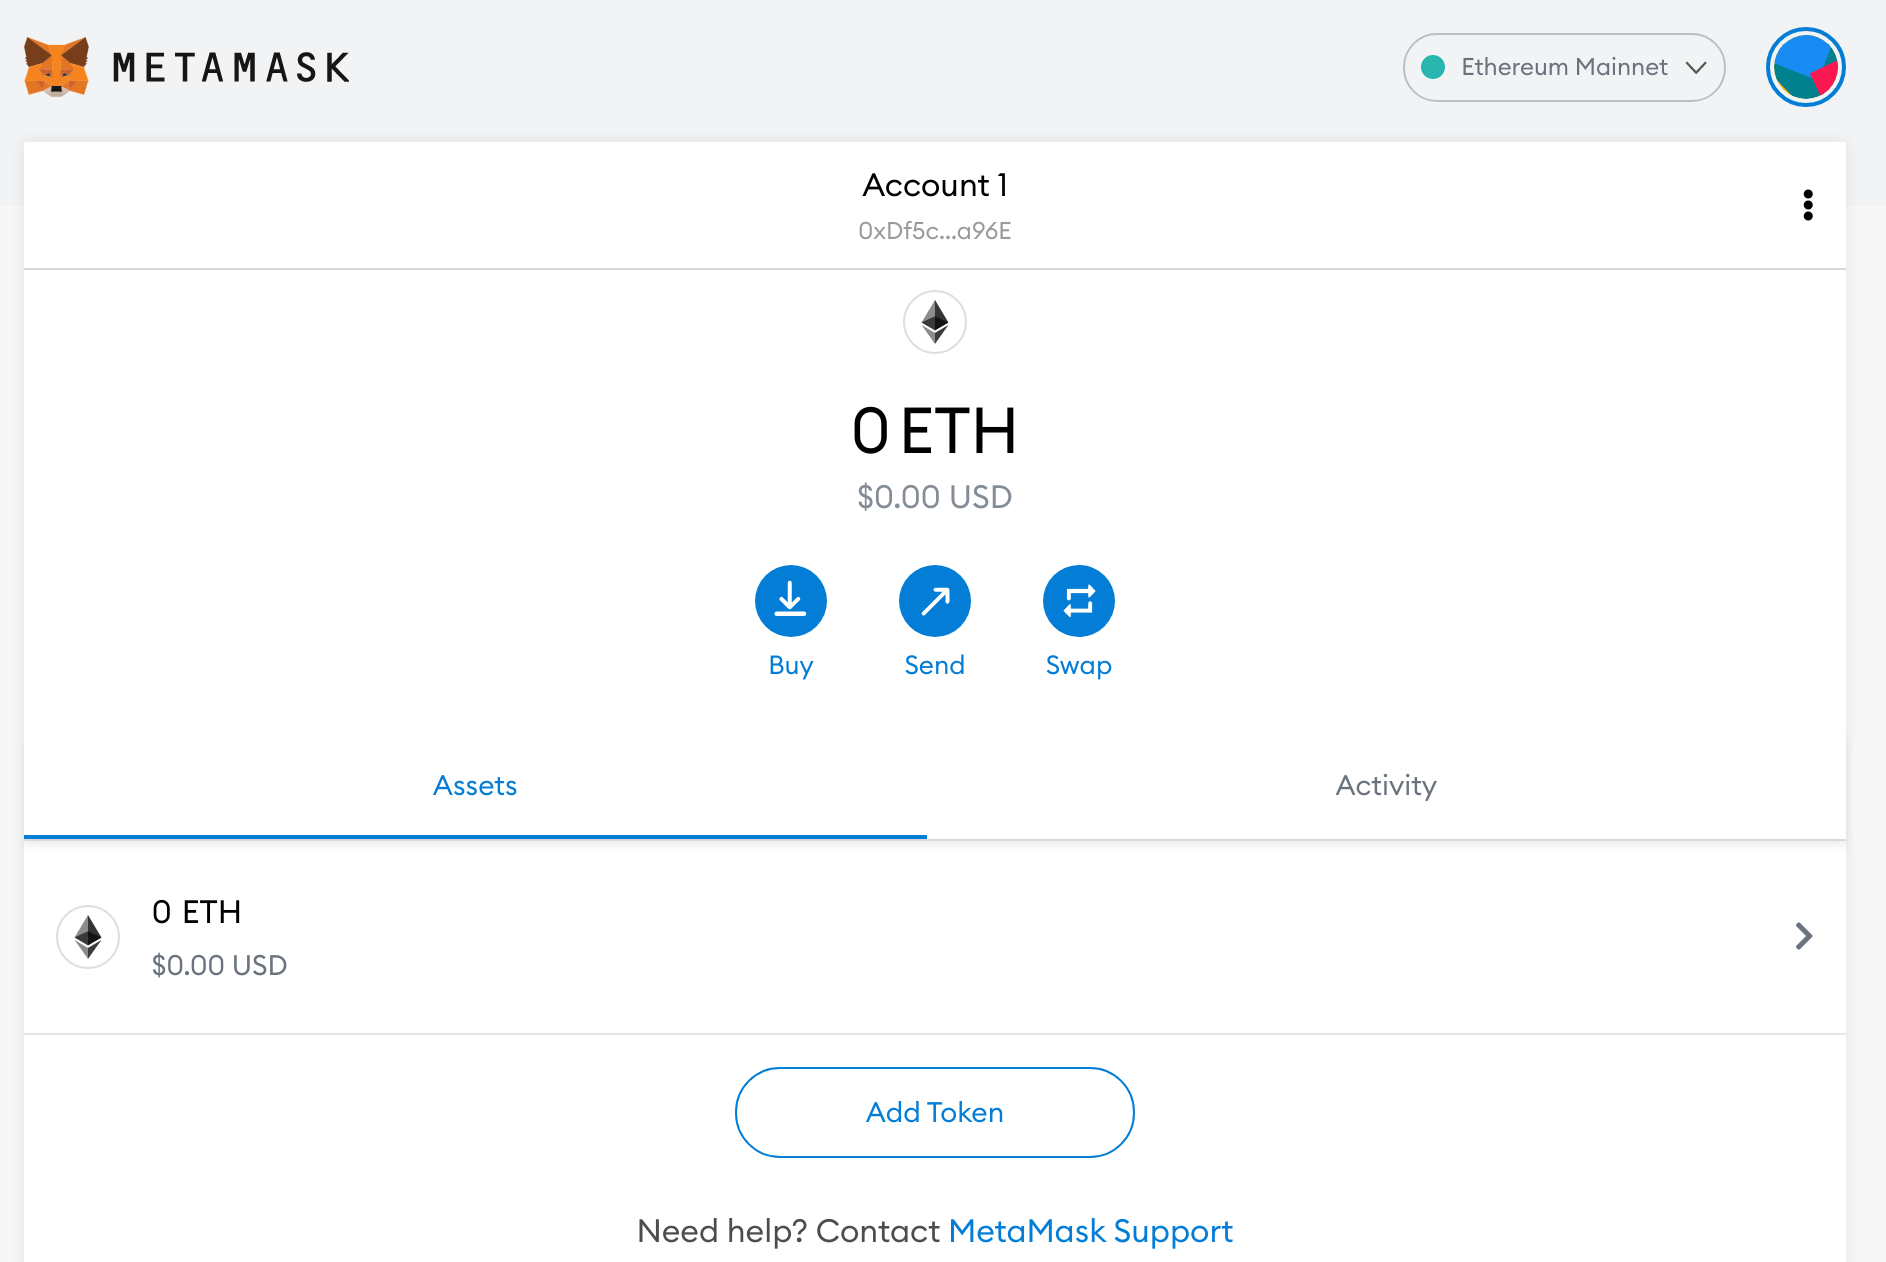
\includegraphics[width=10cm]{../pics/ethereum/metamask-new-account}
	\end{figure}
}

\frame{
	\frametitle{Switch to the Ropsten test network}
	\begin{figure}
		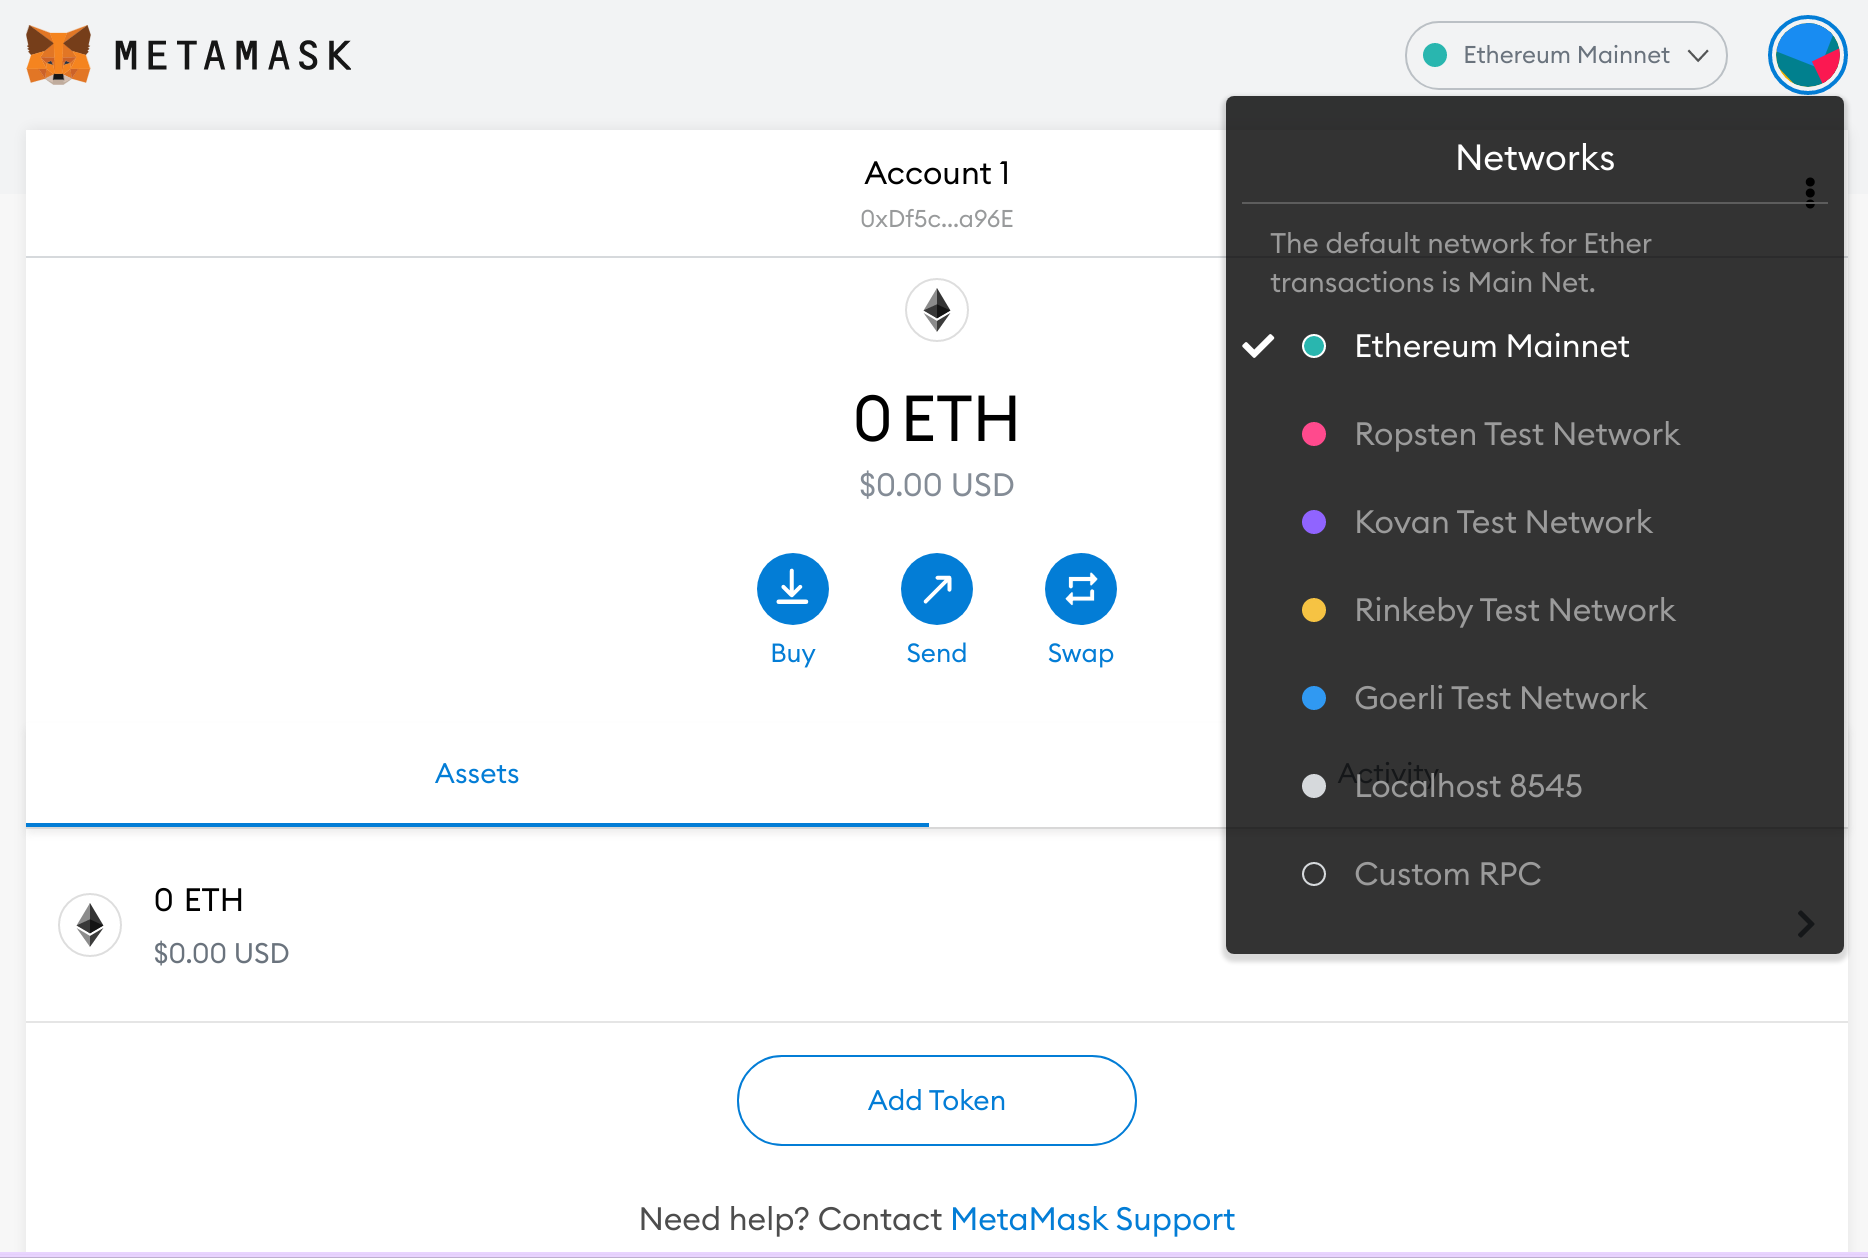
\includegraphics[width=10cm]{../pics/ethereum/metamask-networks}
	\end{figure}
}

\frame{
	\frametitle{Request Ether from the faucet (on the Ropsten network)}
	\framesubtitle{Do it several times; then donate 1 ether to the faucet}
	\begin{figure}
		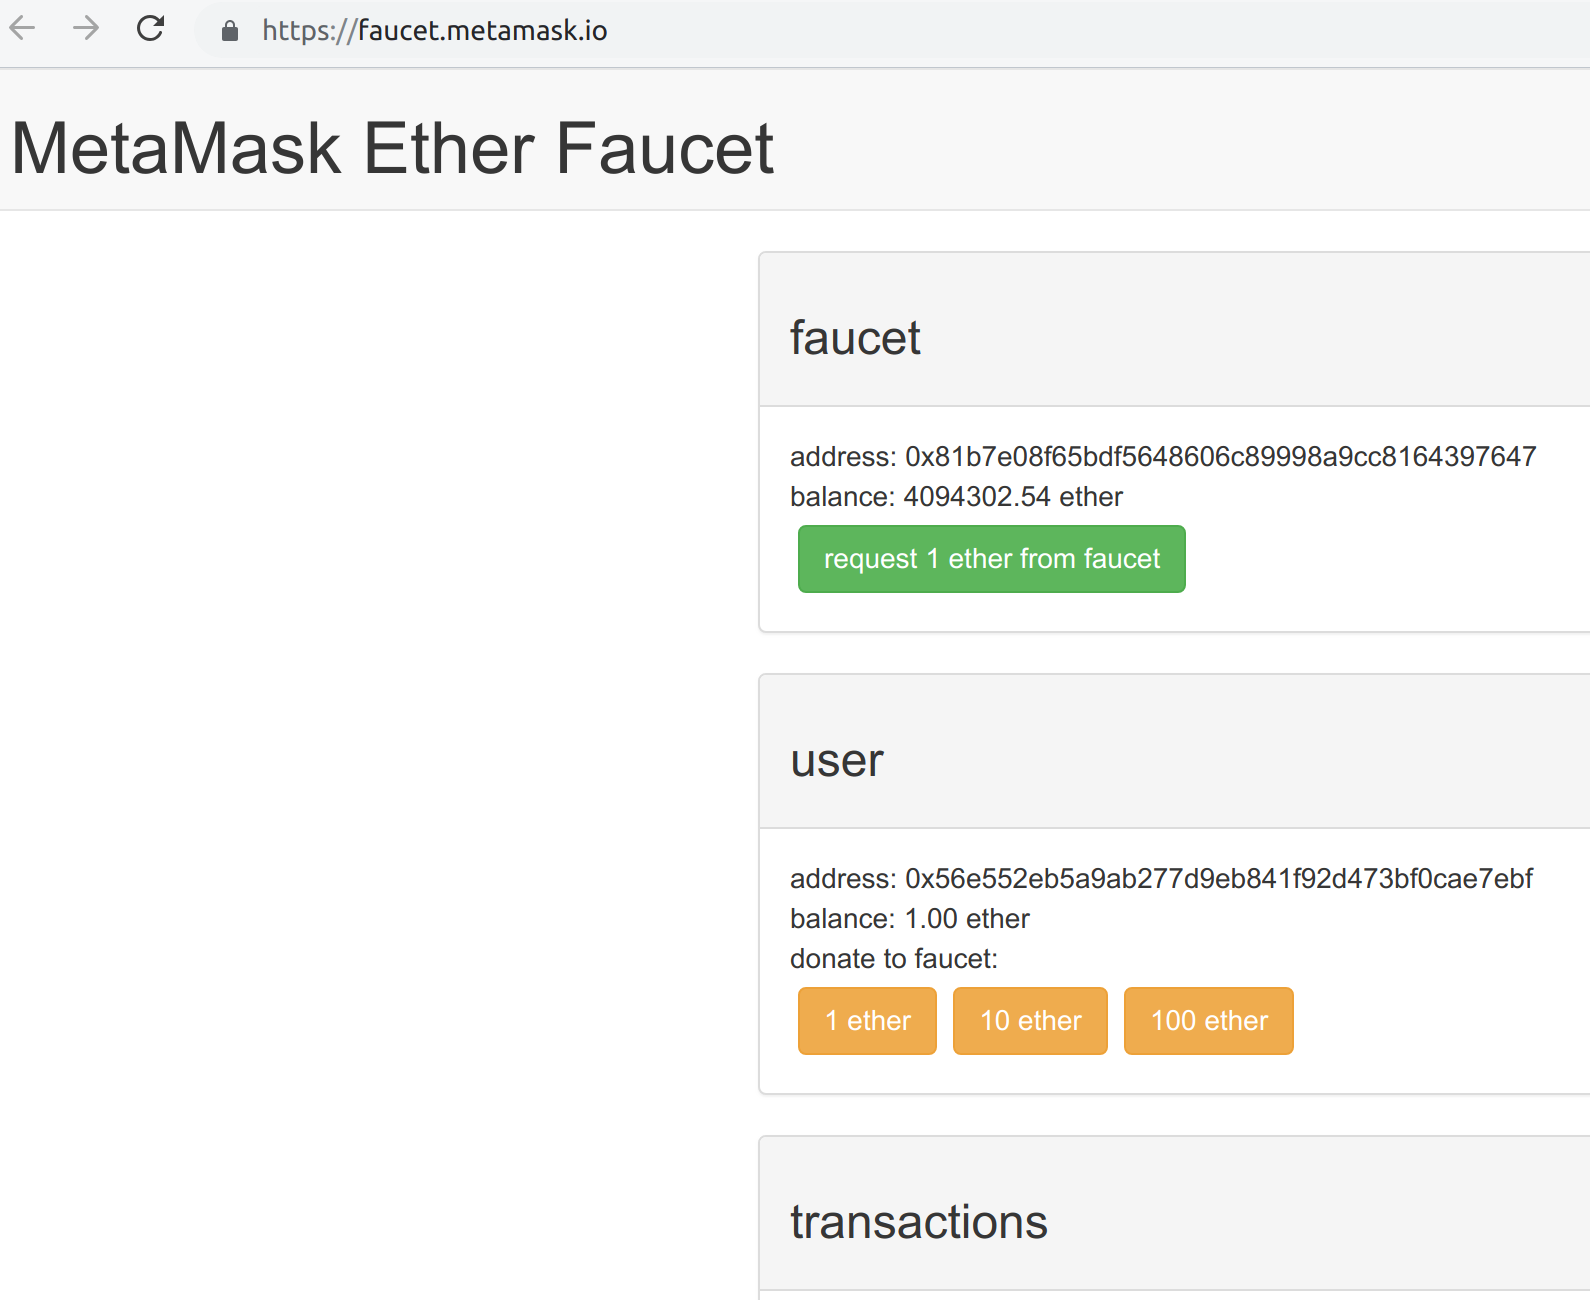
\includegraphics[width=10cm]{../pics/ethereum/faucet-ropsten}
	\end{figure}
}

\frame{
	\frametitle{Check the transaction on Metamask}
	\framesubtitle{Click on the transaction for a detailed view}
	\begin{figure}
		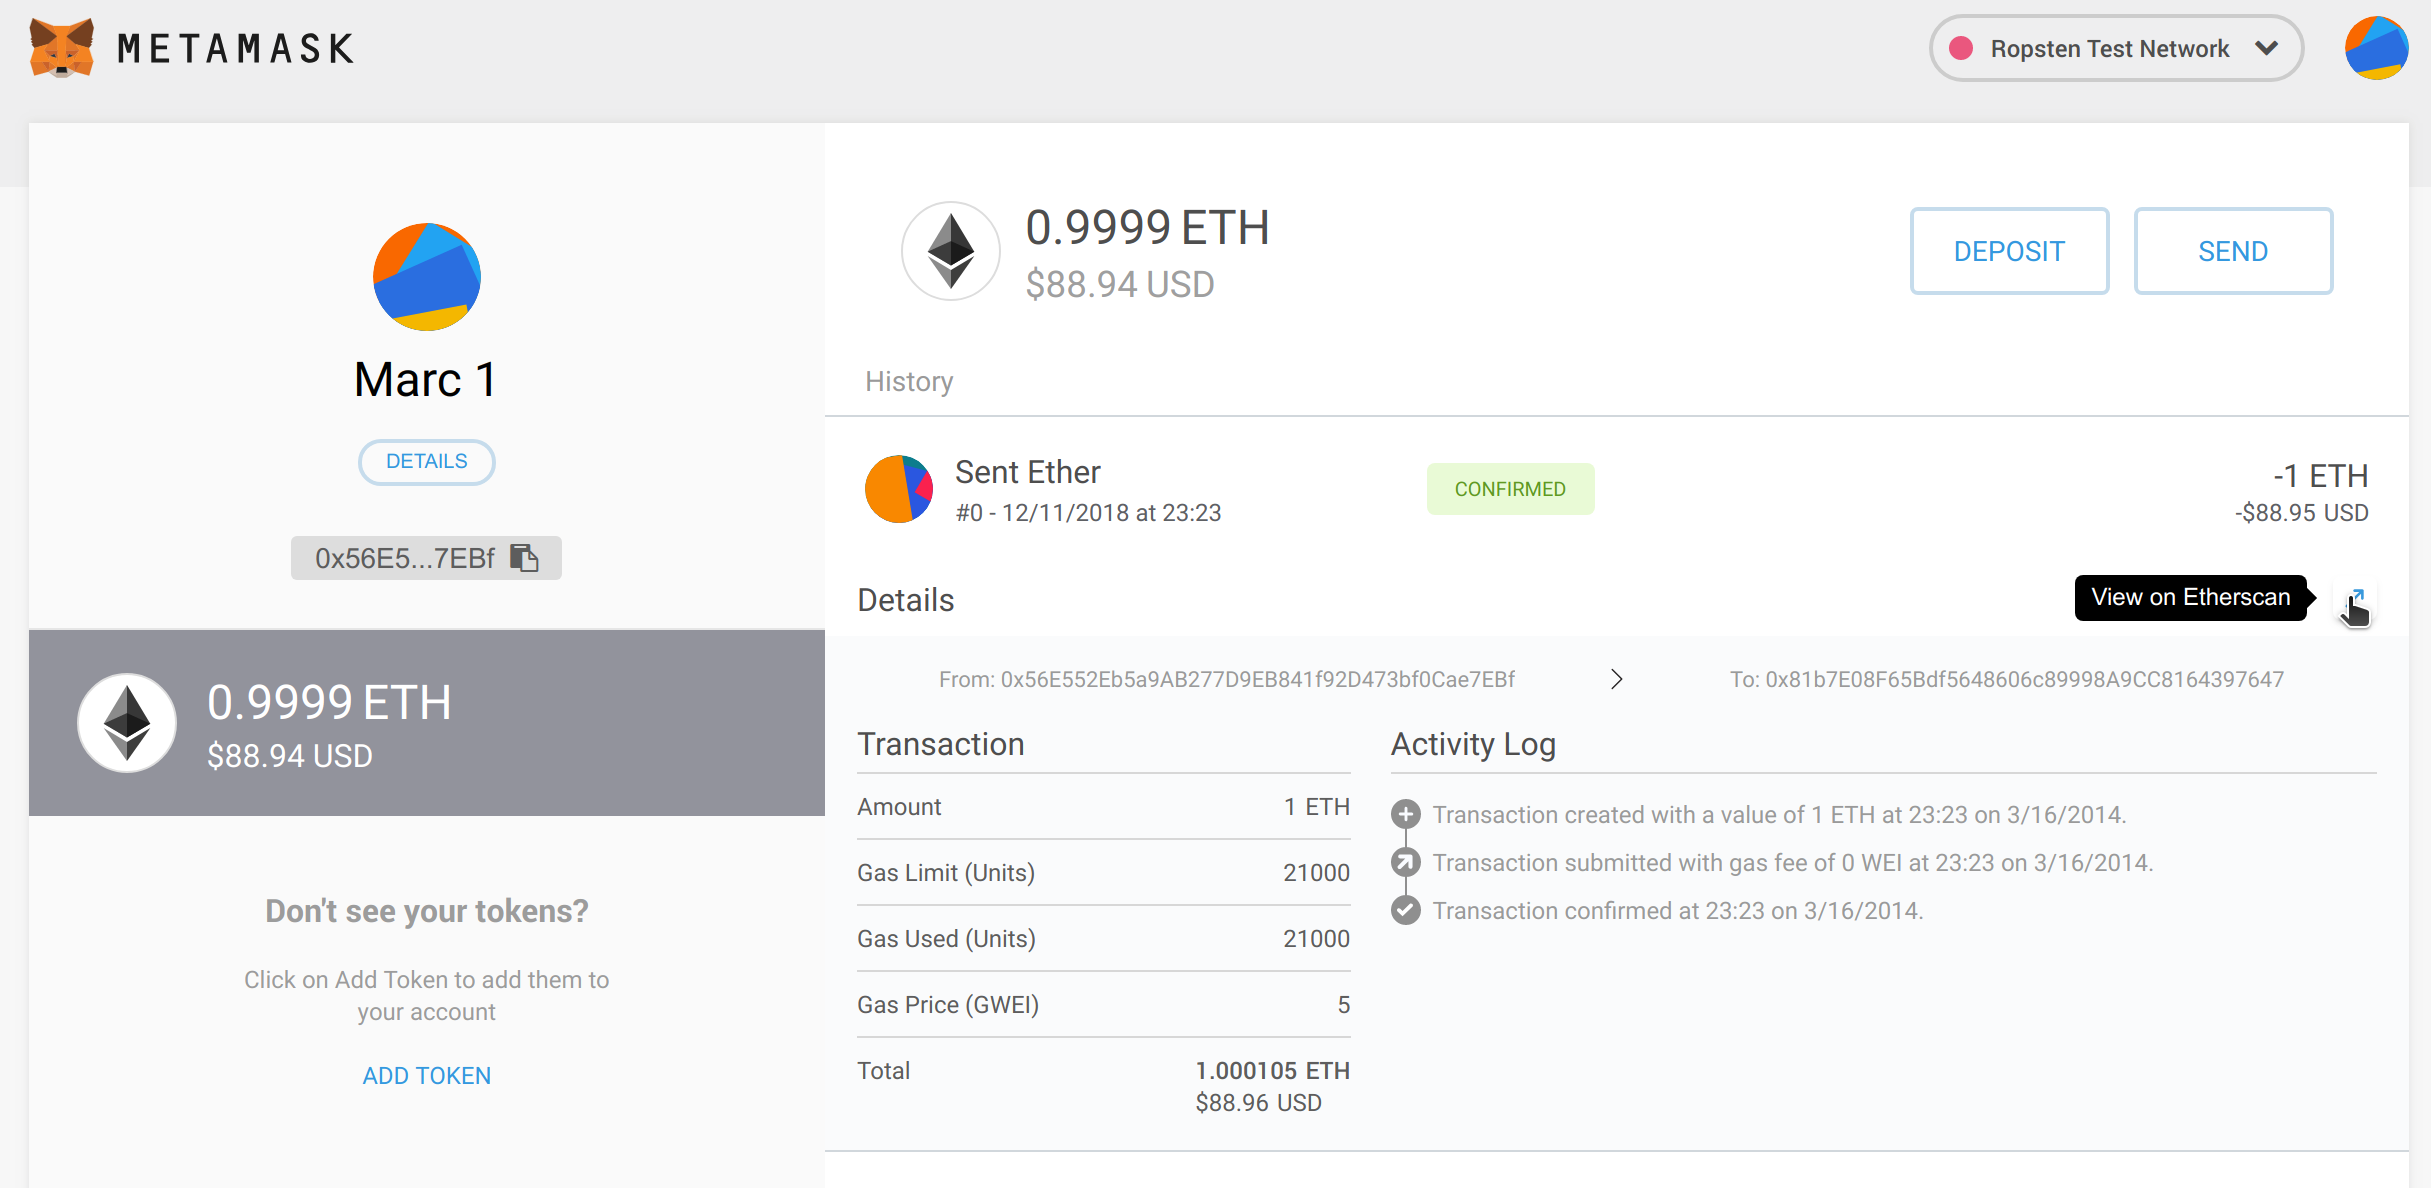
\includegraphics[width=10cm]{../pics/ethereum/metamask-tx-pane-2018}
	\end{figure}
}

\frame{
	\frametitle{Check the transaction on Etherscan}
	\begin{figure}
		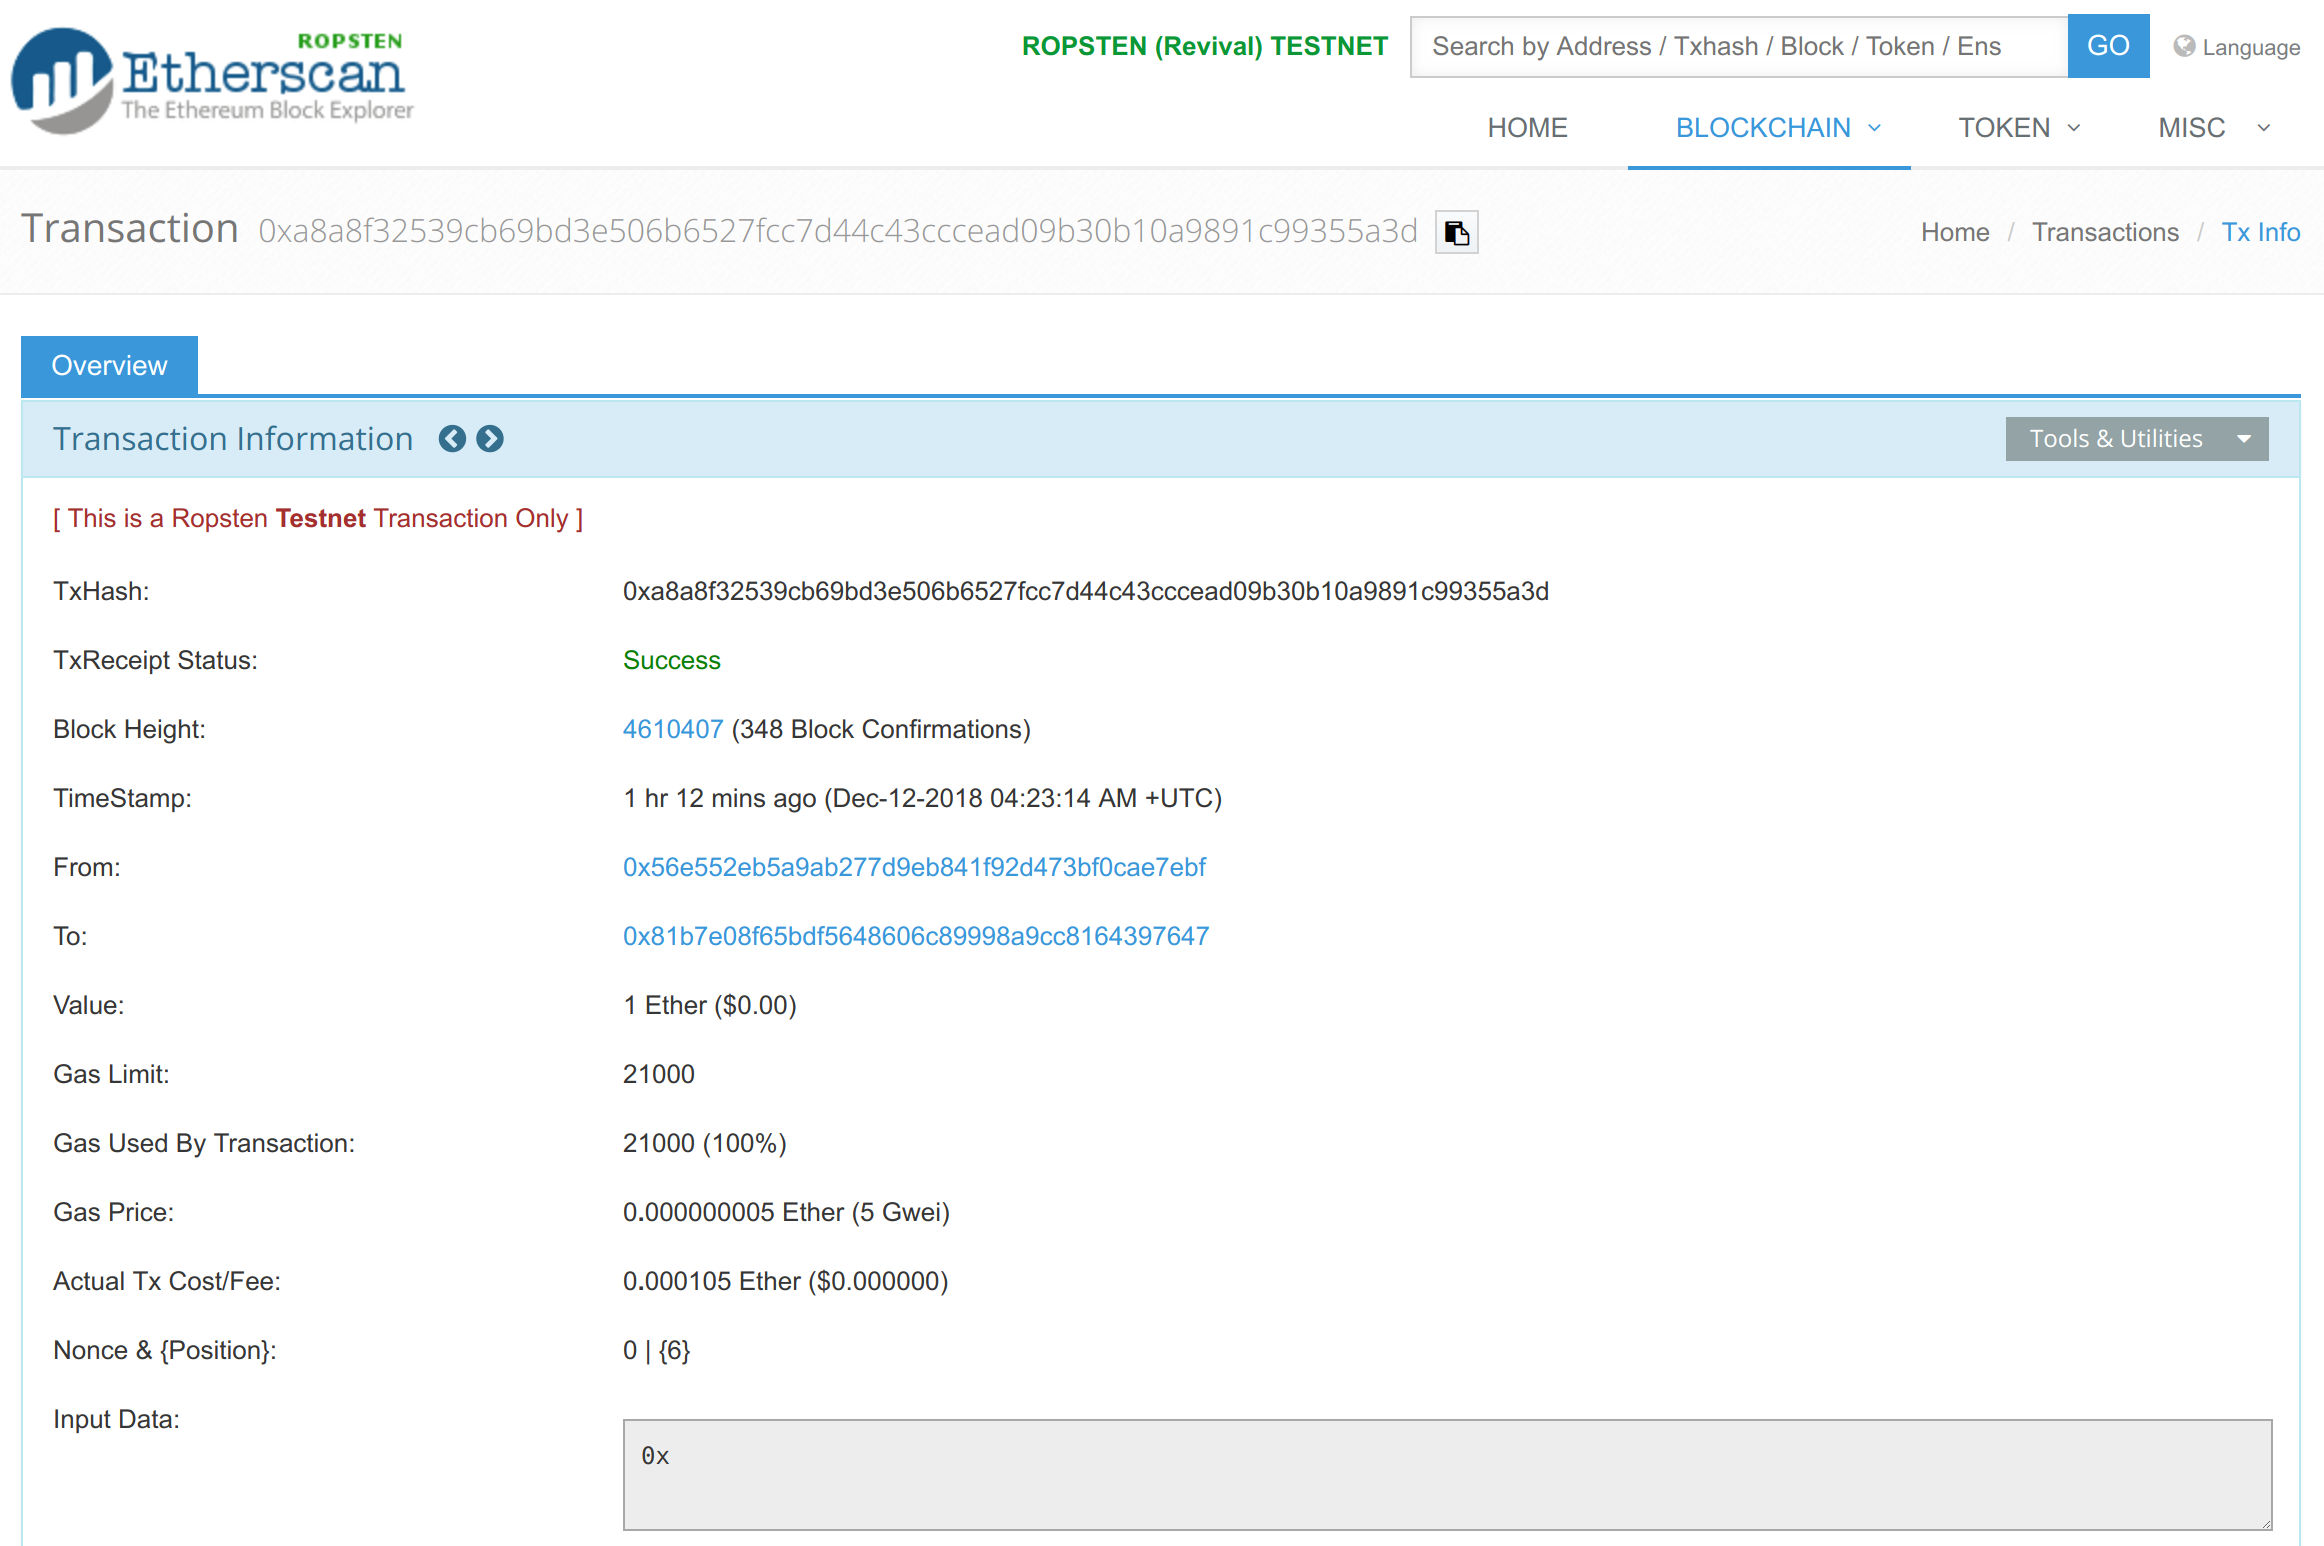
\includegraphics[width=10.9cm]{../pics/ethereum/etherscan-tx-example2}
	\end{figure}
}

\frame{
	\frametitle{A note about gas price}
	\framesubtitle{\url{https://ethgasstation.info}}
	\begin{figure}
		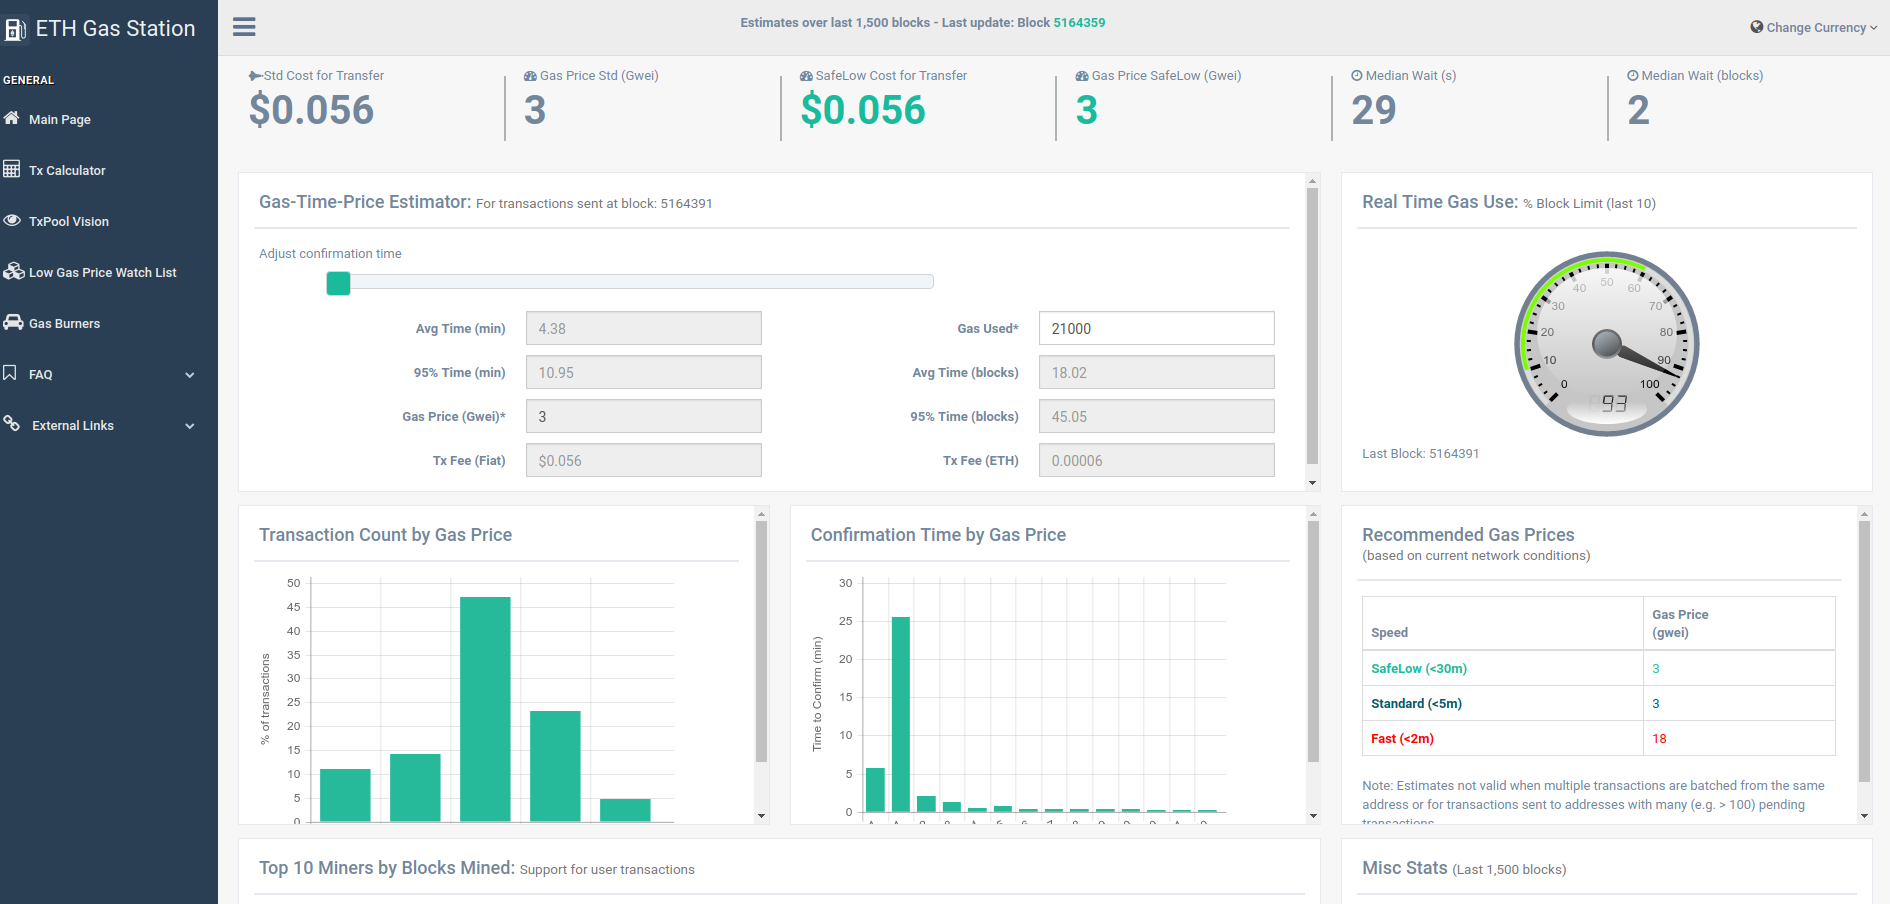
\includegraphics[width=11.5cm]{../pics/ethereum/ethgasstation}
	\end{figure}
}

\frame{
	\frametitle{Price of (real) ether: ETH}
	\framesubtitle{More information: \url{https://www.tradingview.com/symbols/ETHUSD/}}
	\begin{figure}
		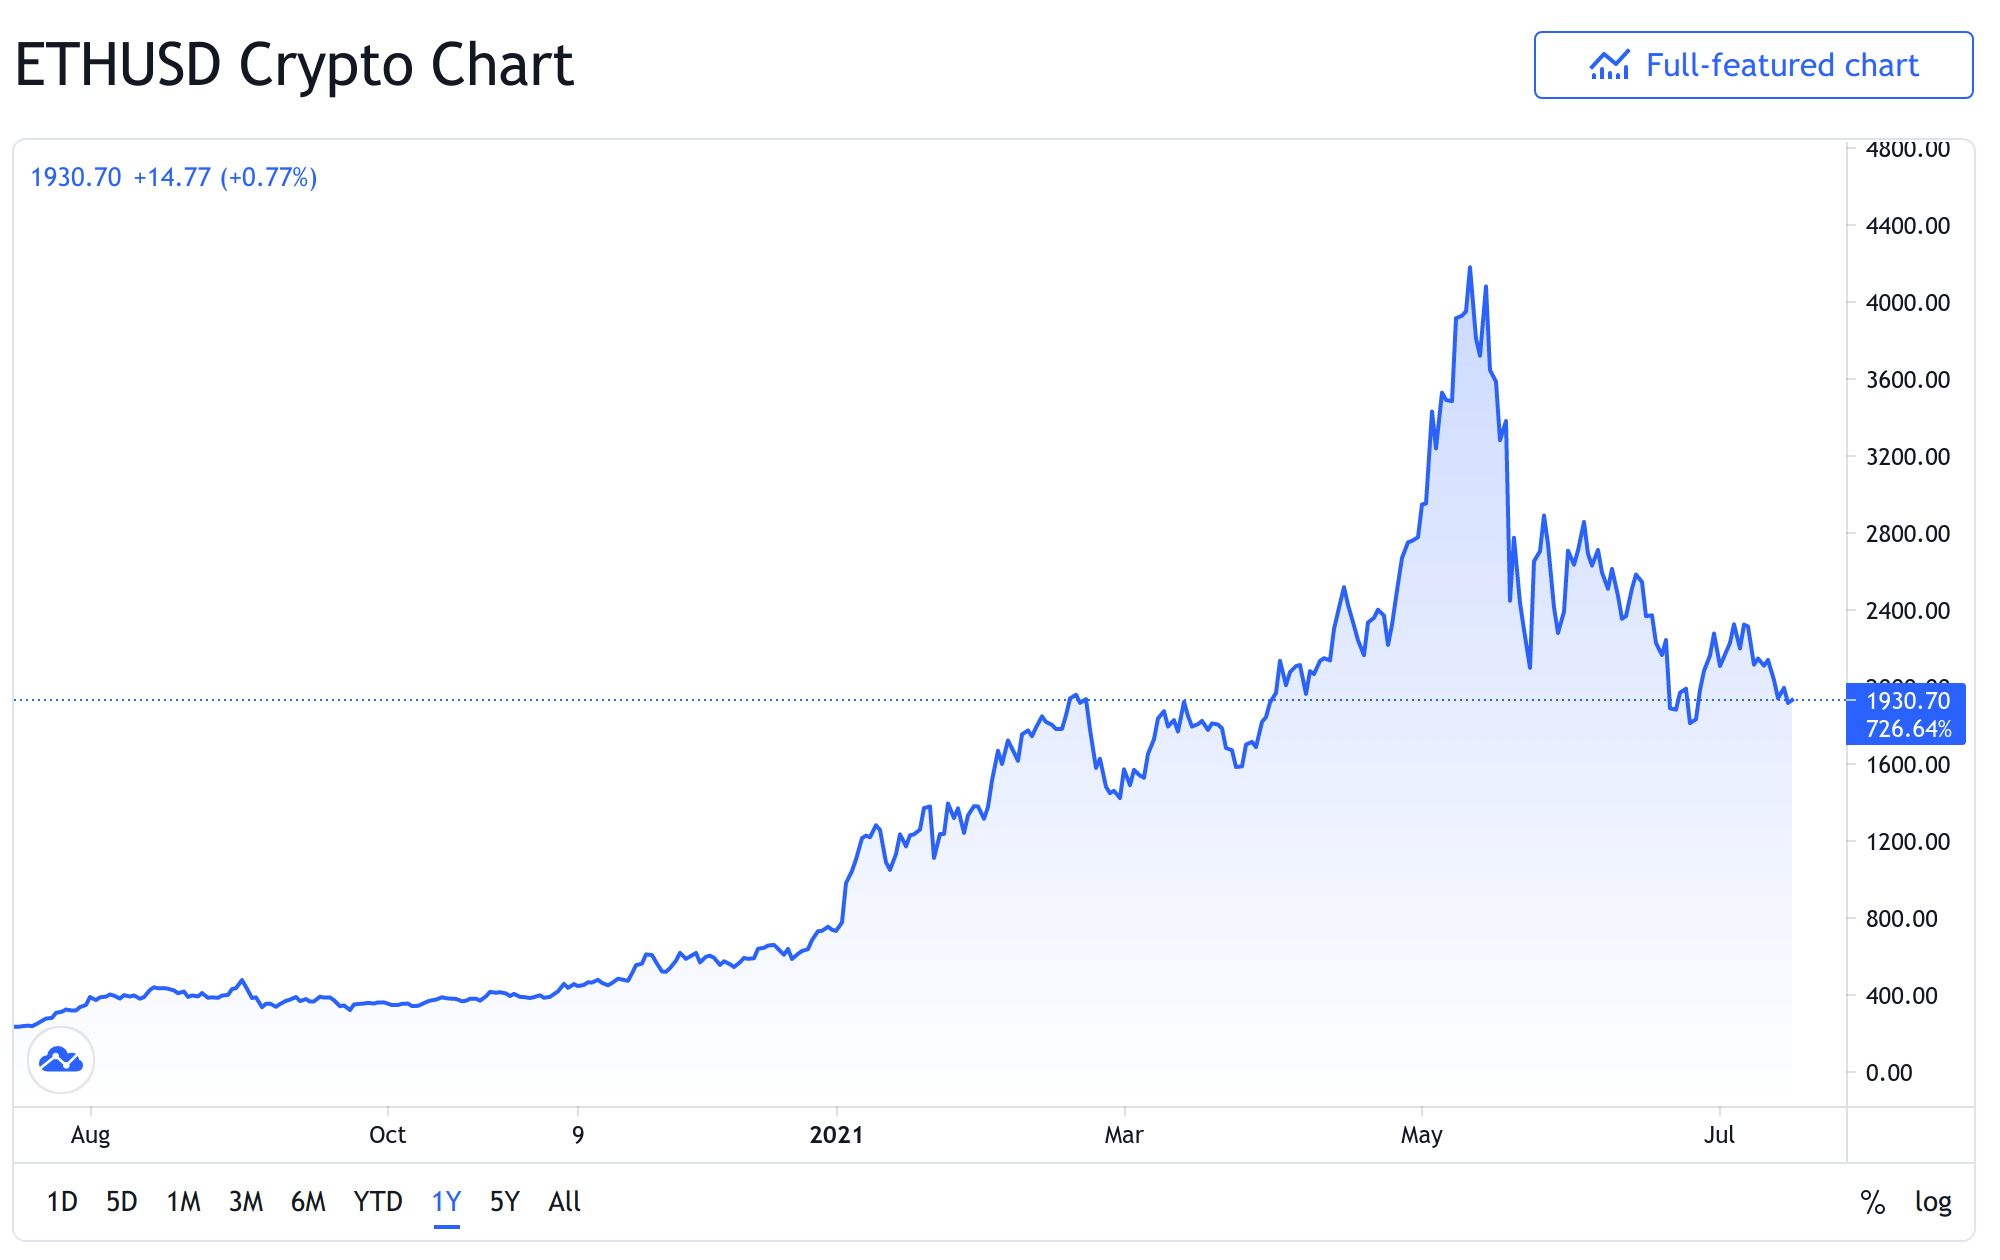
\includegraphics[width=10cm]{../pics/ethereum/ETH-USD-2021-07-16}
	\end{figure}
}

\frame{
	\frametitle{Wallets}
	\framesubtitle{More information: \url{https://blockgeeks.com/guides/cryptocurrency-wallet-guide/}}
	\begin{figure}
		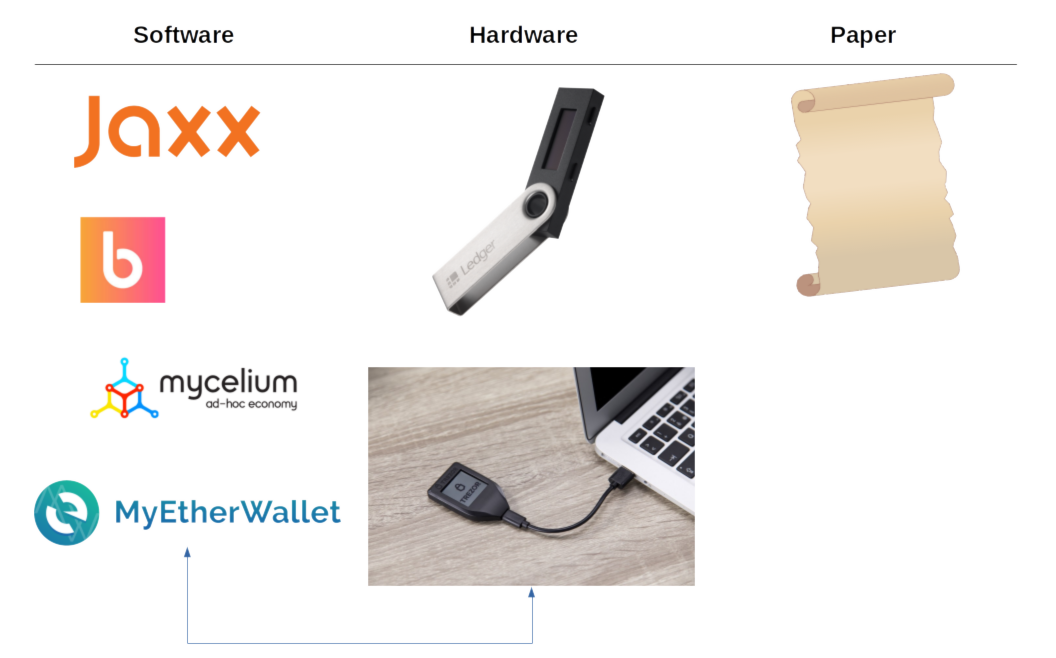
\includegraphics[width=11.5cm]{../pics/ethereum/wallets}
	\end{figure}
}

\frame{
	\frametitle{Exchanges}
	\begin{enumerate}
		\item Centralized Exchanges (Coinbase, Binance, Kraken, eToro, Huobi, ...)
    \item Decentralized Exchanges (DEXes)
	\end{enumerate}
}

\frame{
	\frametitle{Top DEXes}
	\framesubtitle{More information: \url{https://defipulse.com}}
	\begin{figure}
		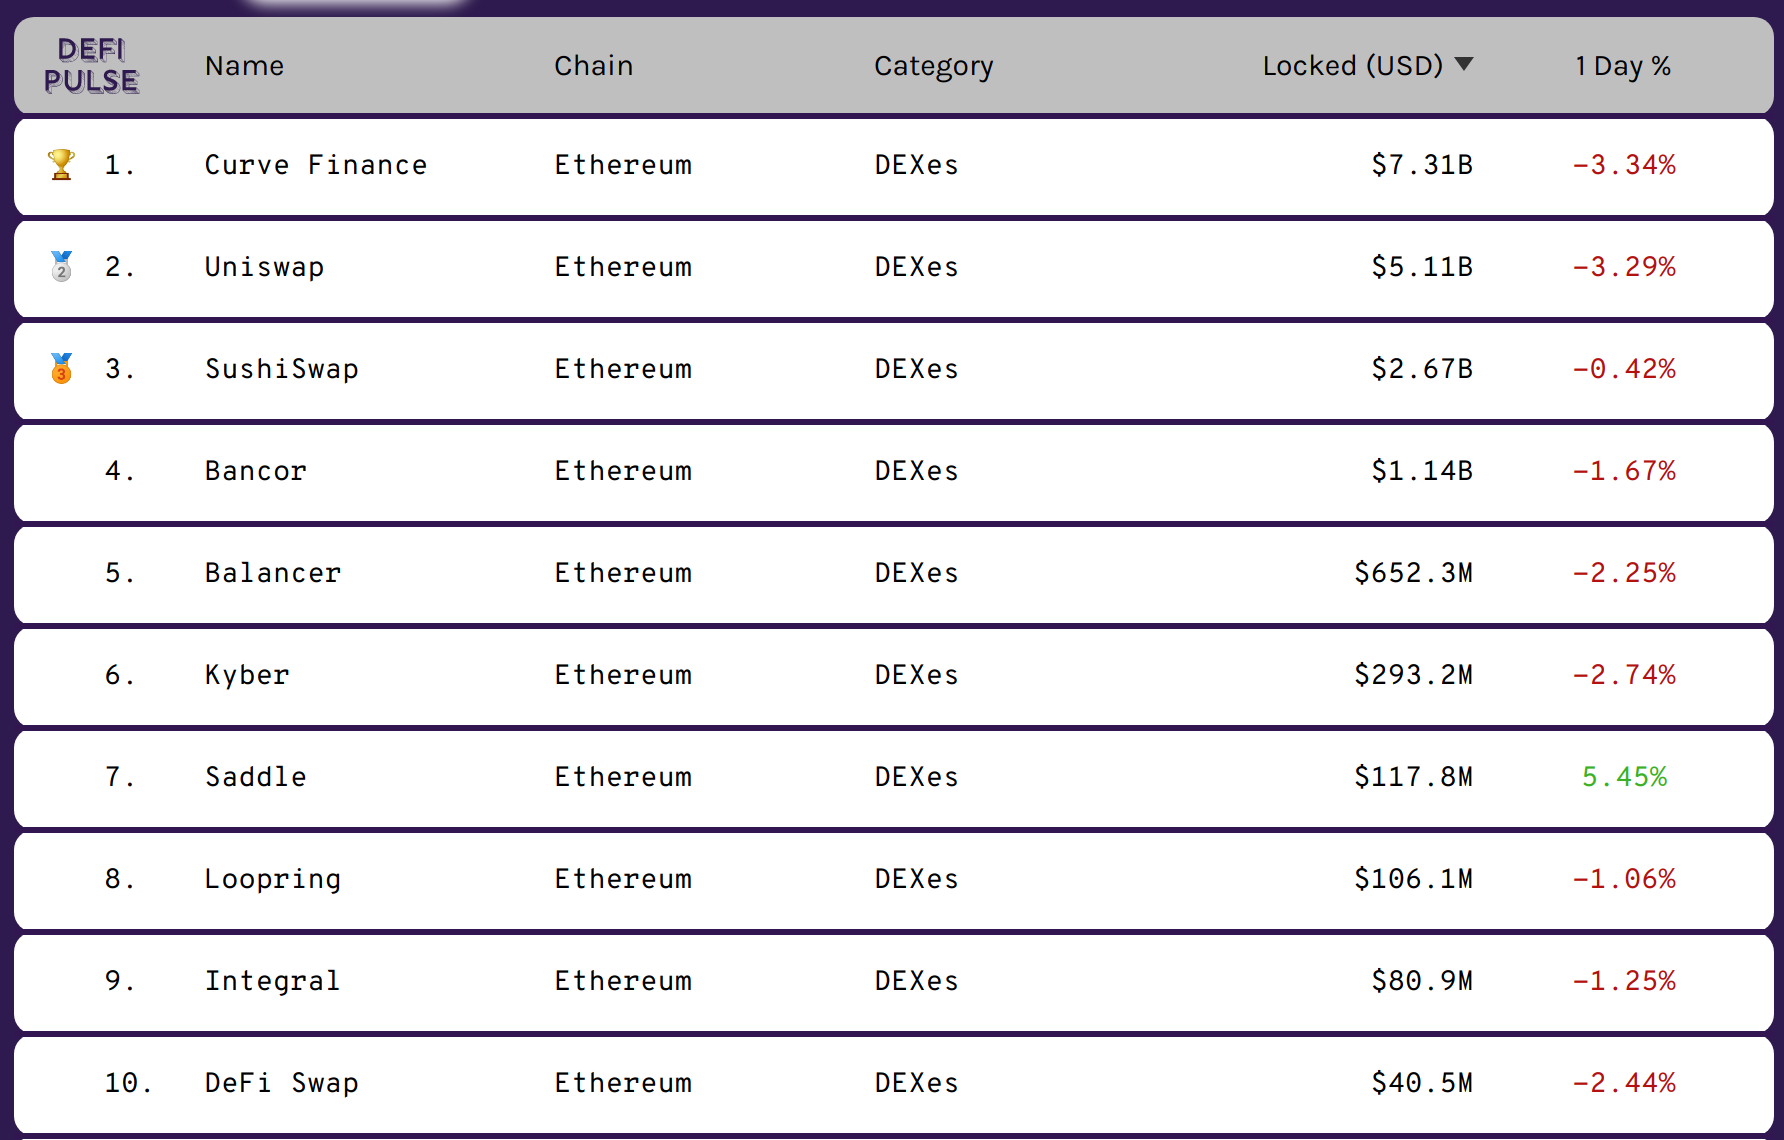
\includegraphics[width=11cm]{../pics/DeFi/DEXes-defi-pulse-2021-07-16}
	\end{figure}
}

\frame{
	\frametitle{ATMs}
	\framesubtitle{More information: \url{https://coinatmradar.com/country/38/bitcoin-atm-canada/}}
	\begin{figure}
		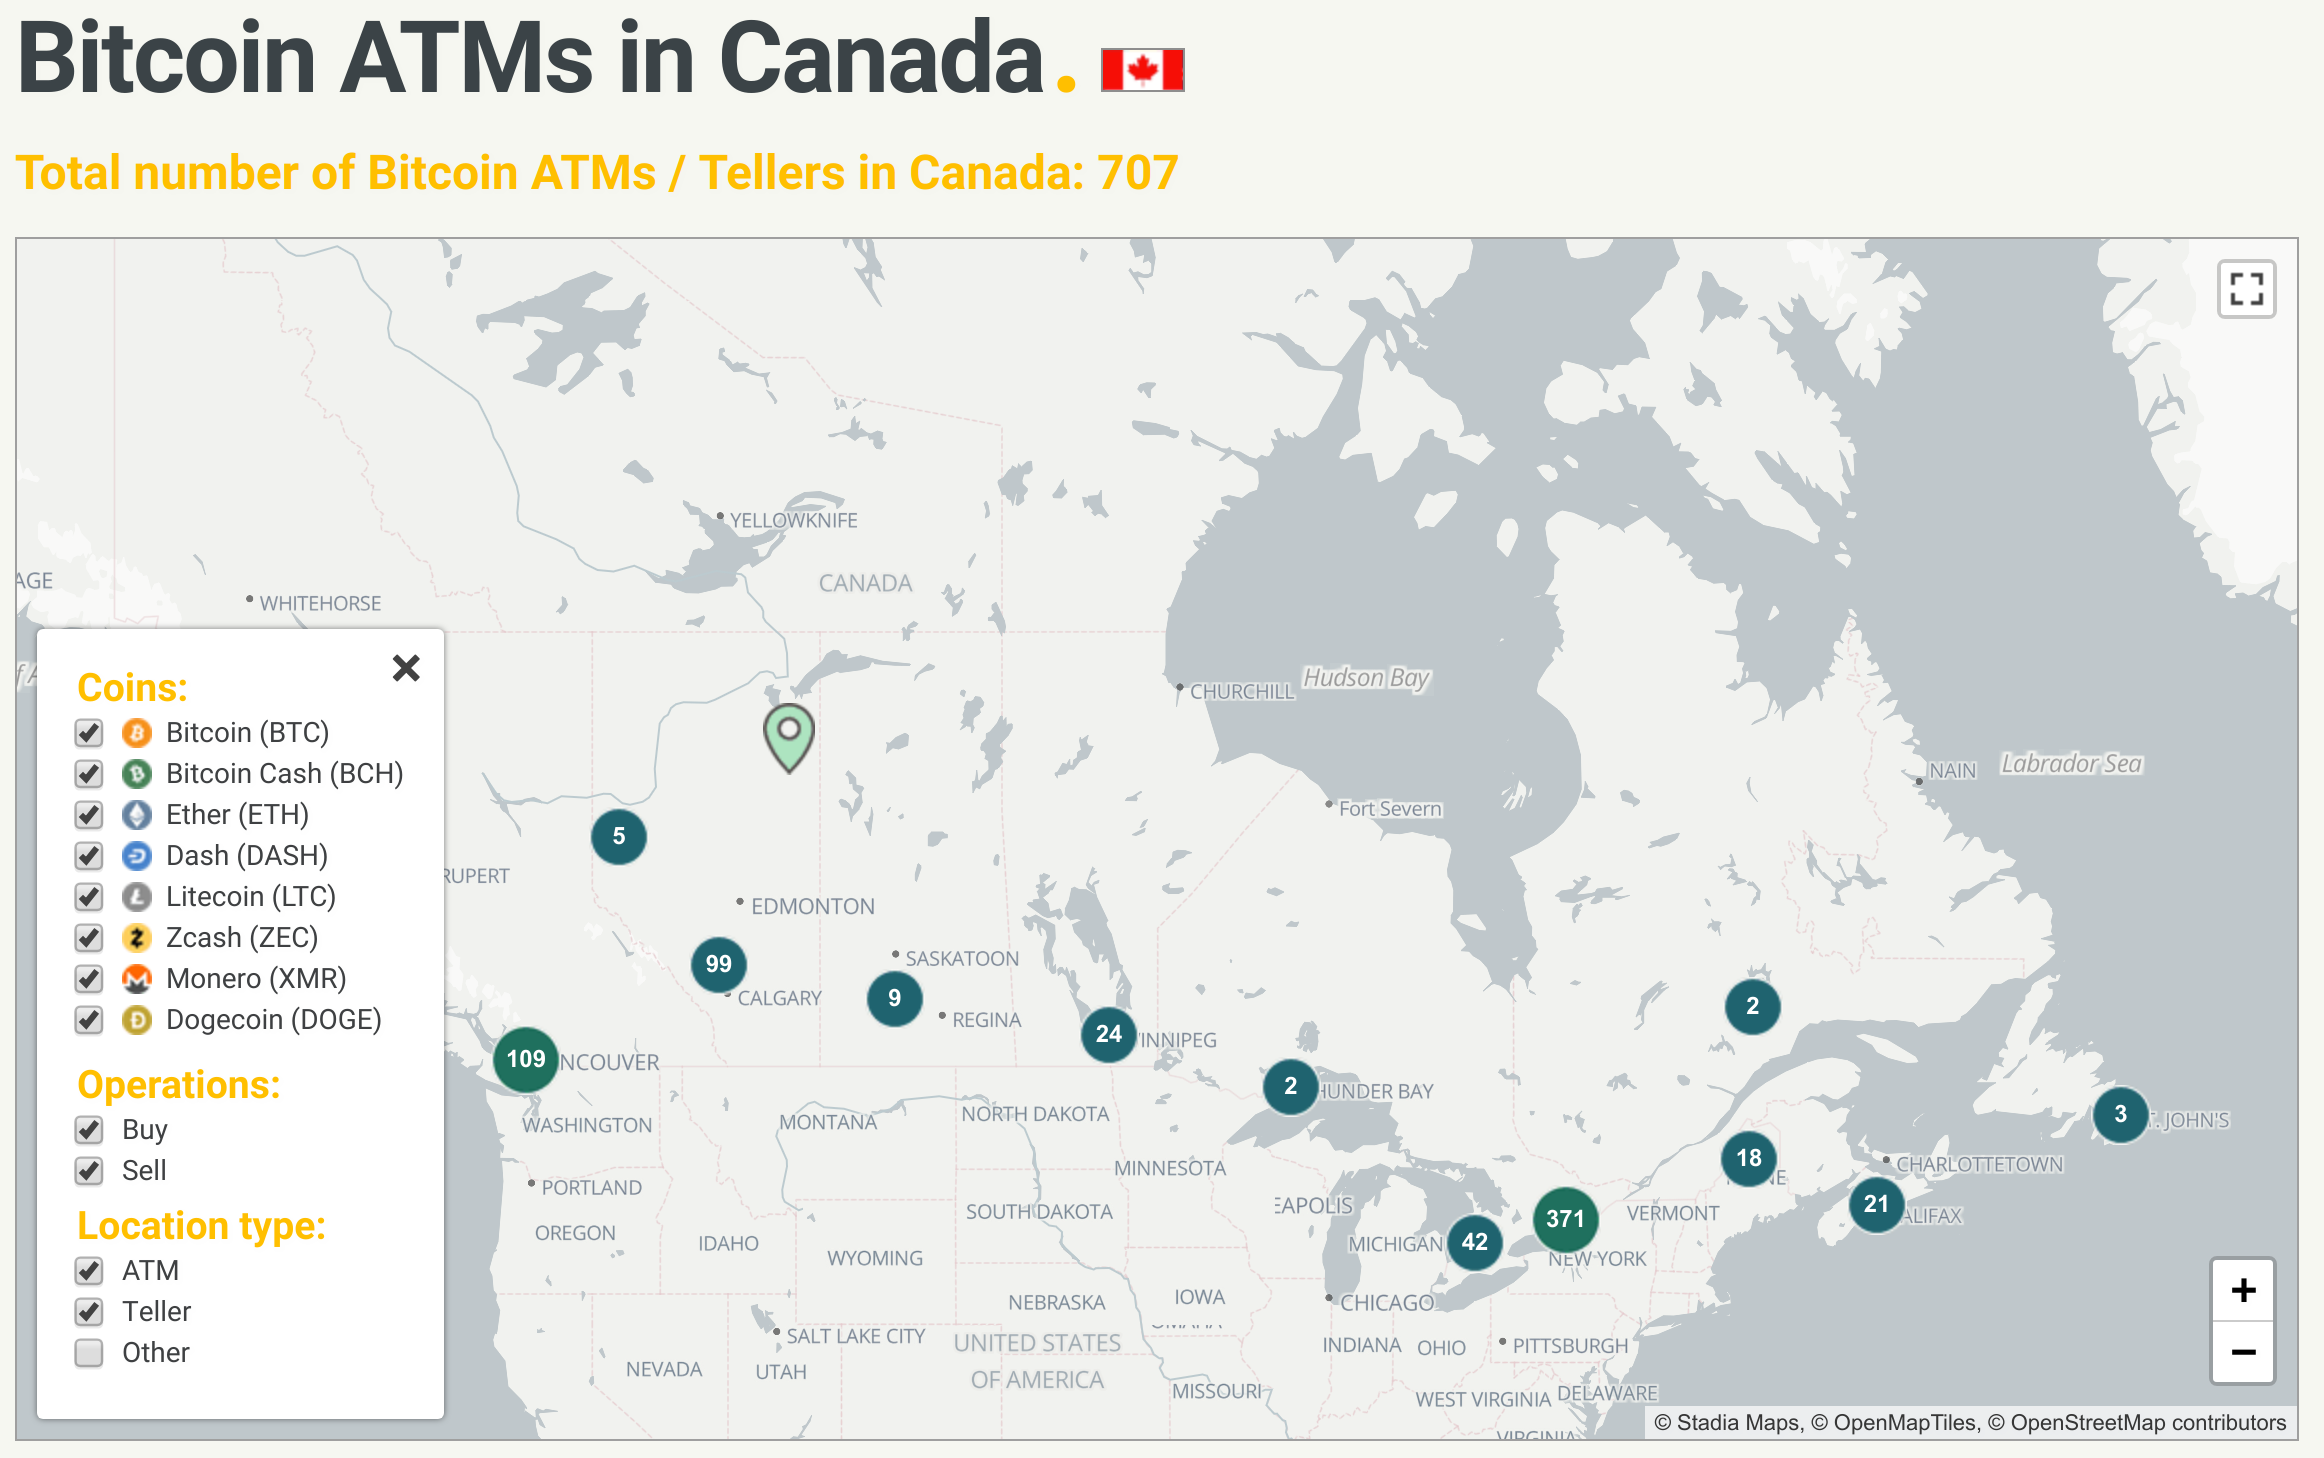
\includegraphics[width=10cm]{../pics/ethereum/bitcoin-atms-canada-2019-01}
	\end{figure}
}

\frame{
	\frametitle{ATMs}
	\framesubtitle{More information: \url{https://coinatmradar.com/country/38/bitcoin-atm-canada/}}
	\begin{figure}
		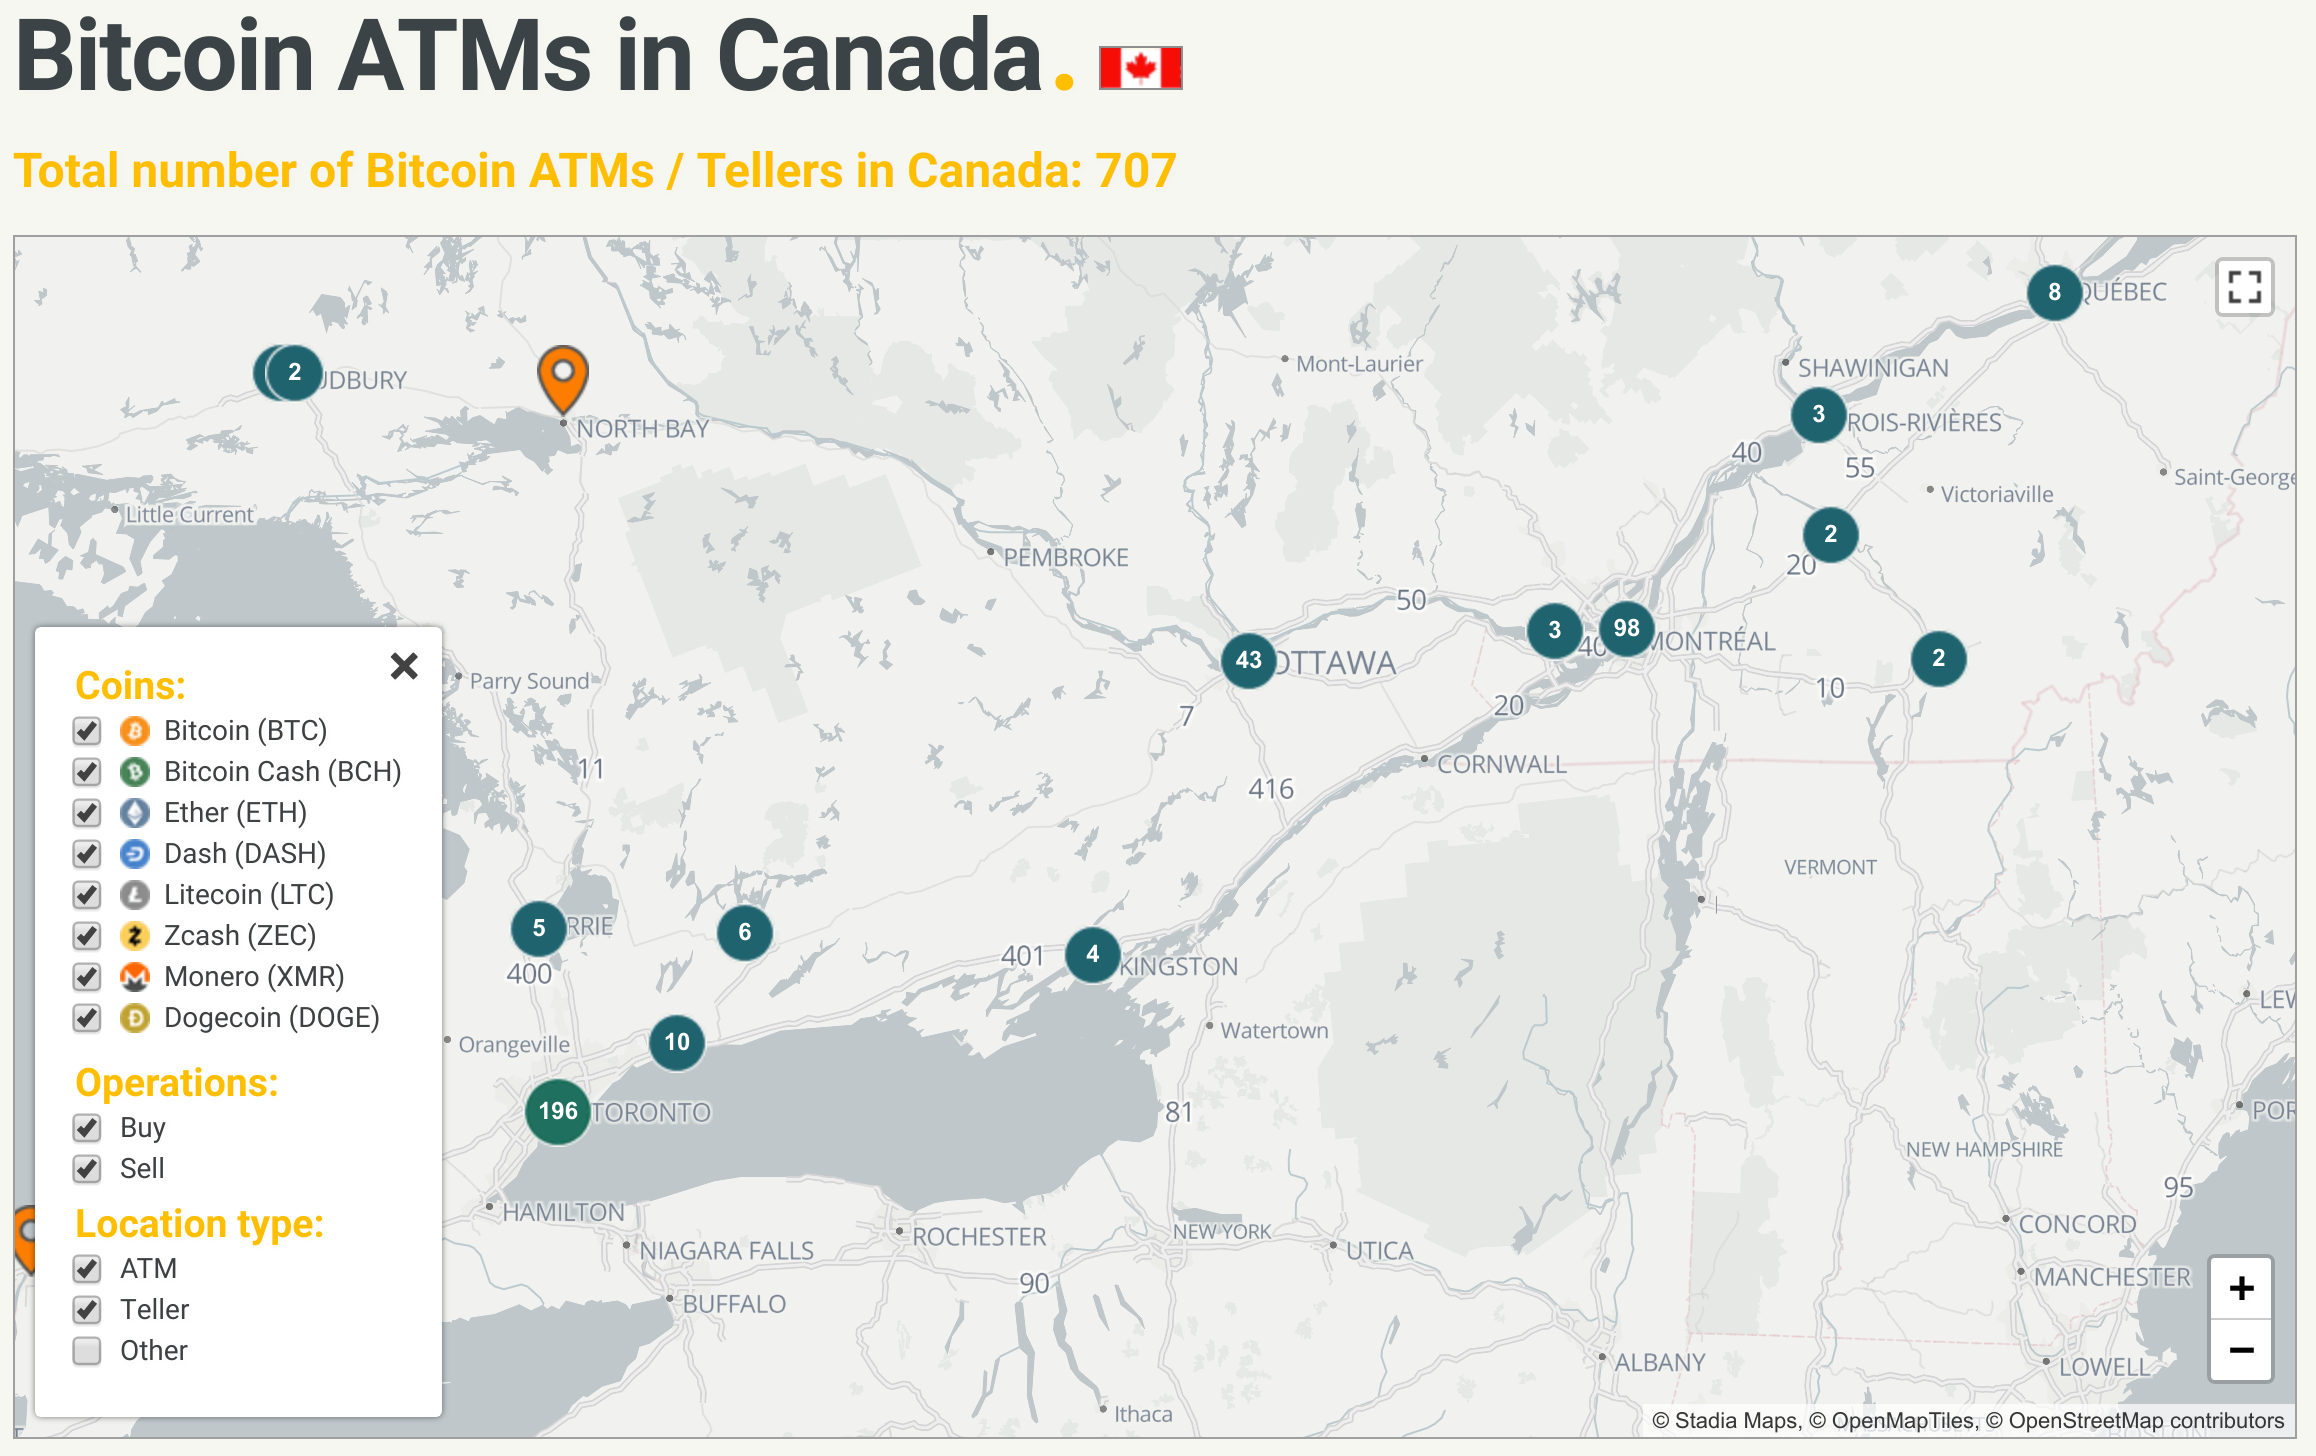
\includegraphics[width=10cm]{../pics/ethereum/bitcoin-atms-ontario-quebec-2019-01}
	\end{figure}
}

\frame{
	\frametitle{Other crypto-assets}
	\framesubtitle{More information: \url{https://www.tradingview.com/markets/cryptocurrencies/prices-all/}}
	\begin{figure}
		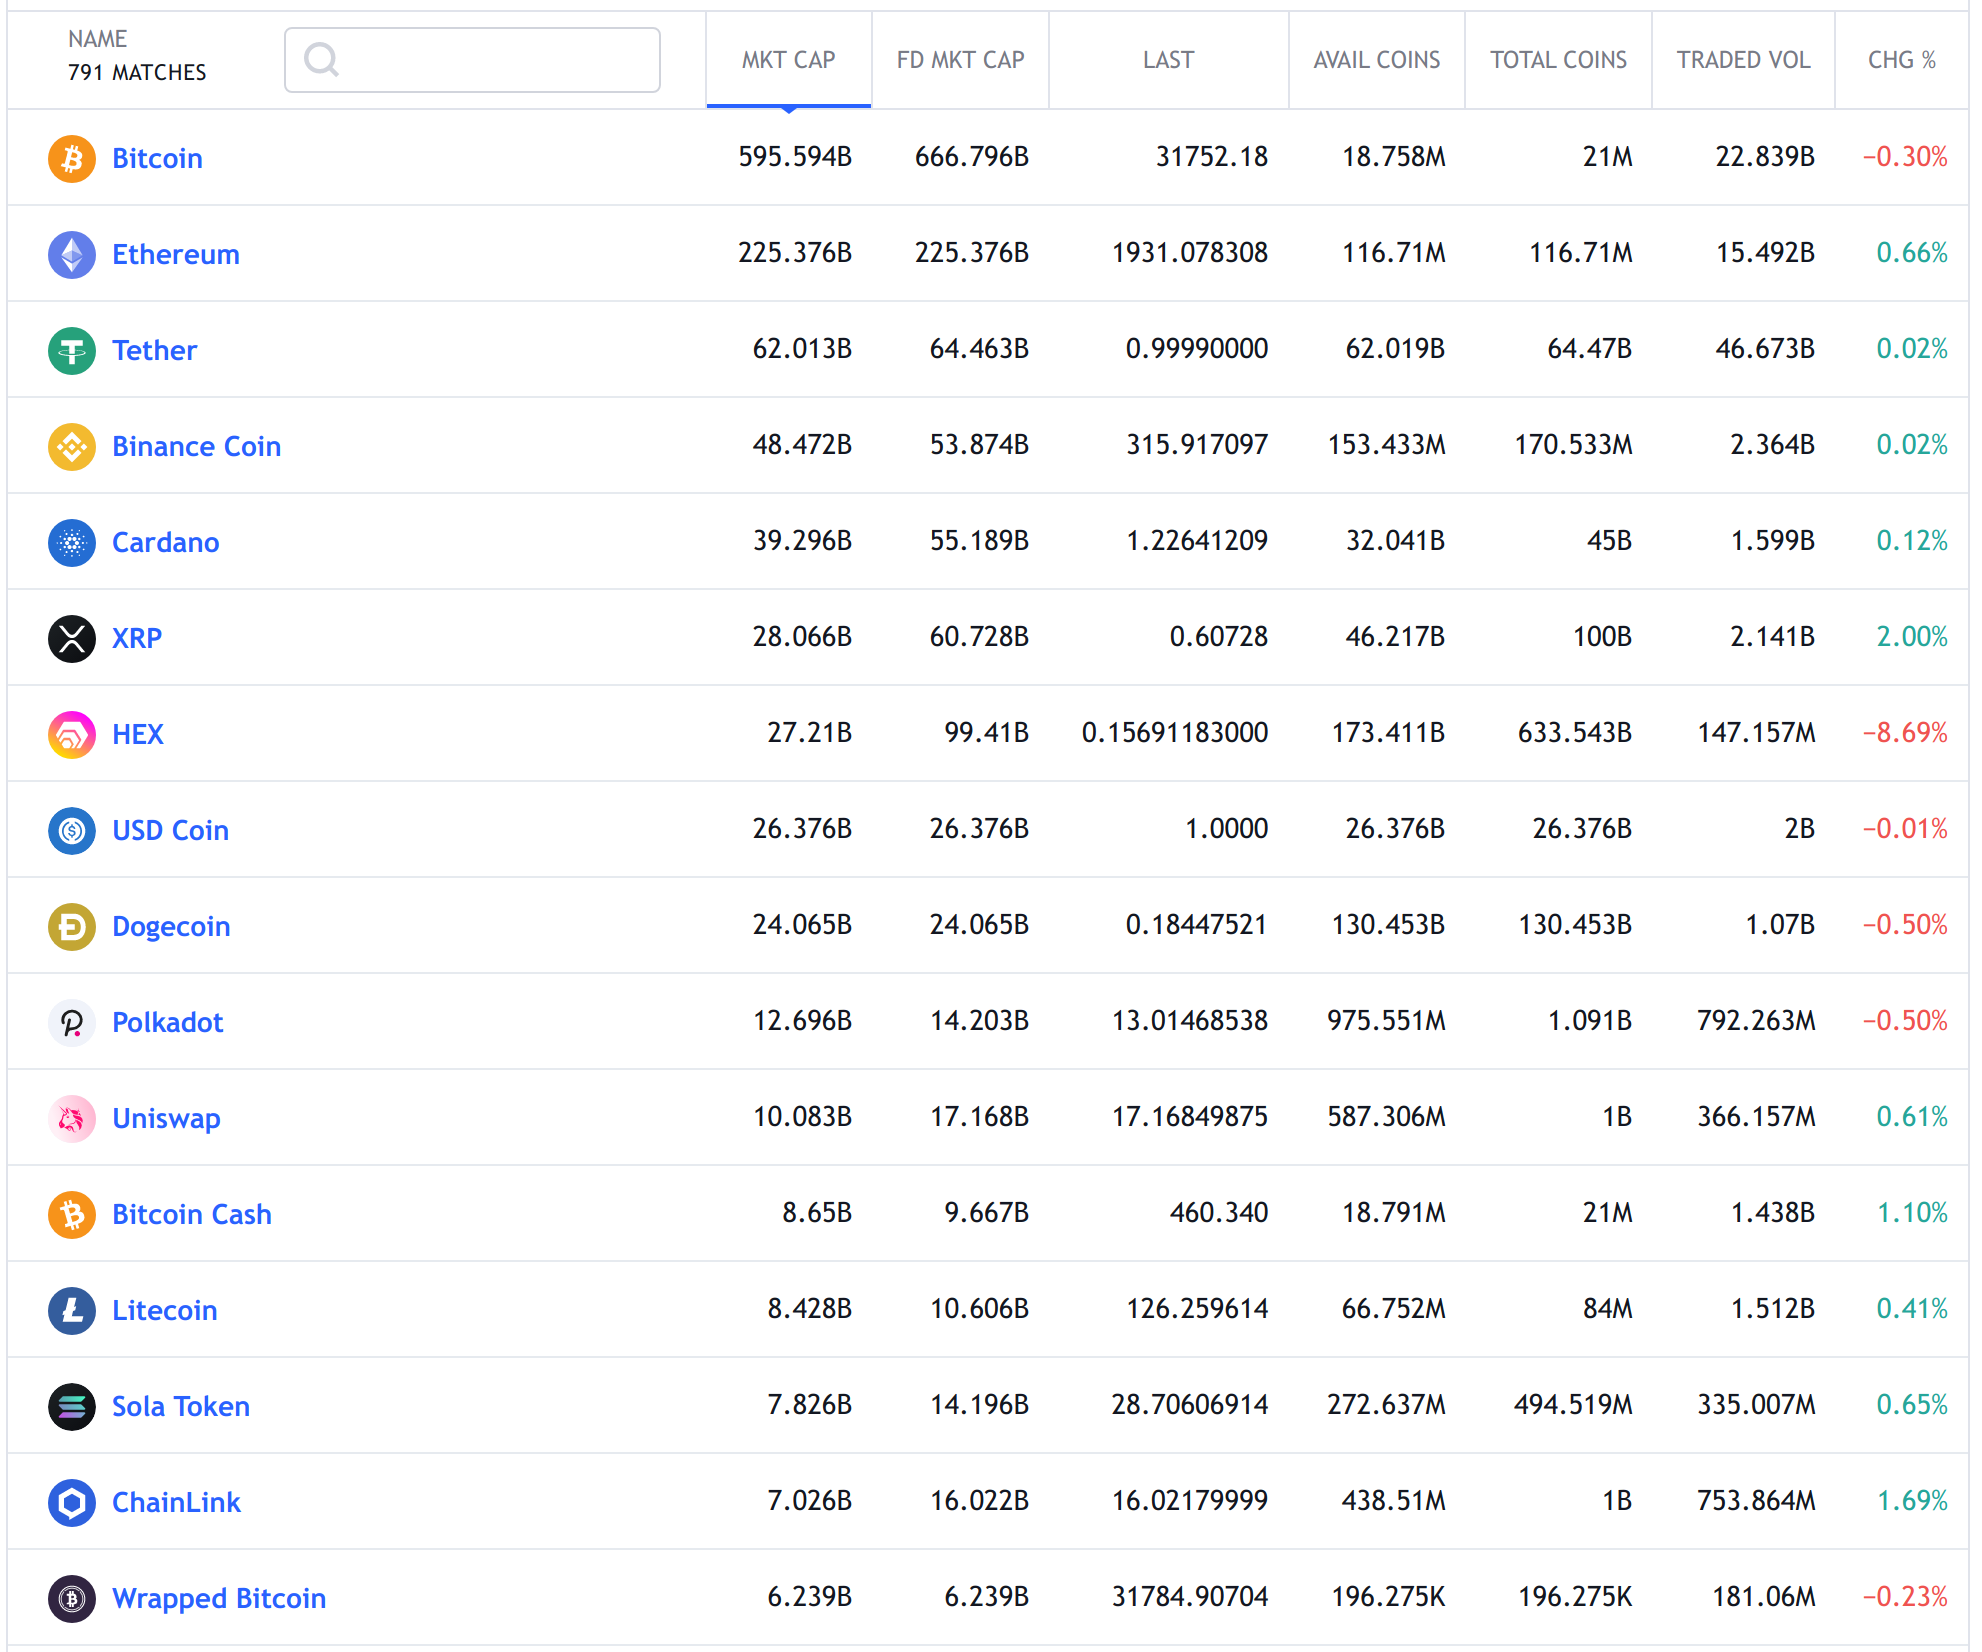
\includegraphics[width=10cm]{../pics/DeFi/crypto-coins-2021-07-16}
	\end{figure}
}


% ======================================================================================================
%                         Mint your own token (the easy way)
% ======================================================================================================
\section{Create your own token}
\subsection{The easy way}
\frame{
	\frametitle{}
	\centering\Huge
	Let's create your own token!
}

\frame{
	\frametitle{Create your own (ERC-20) token}
	\begin{figure}
		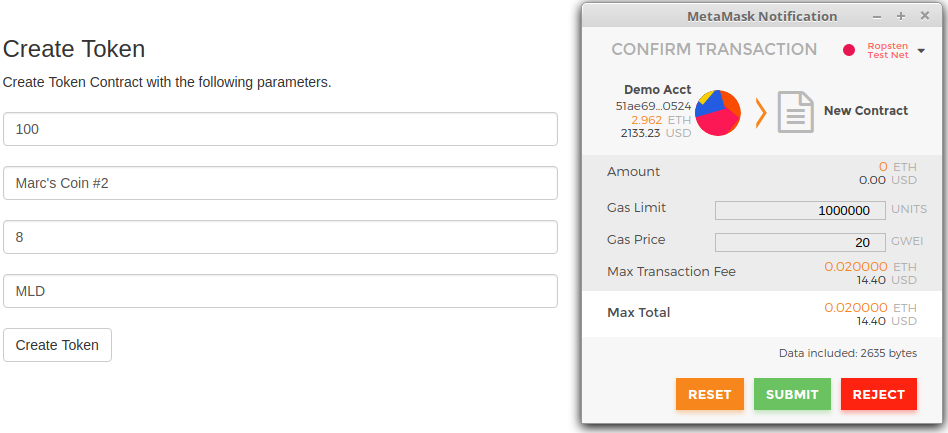
\includegraphics[width=10cm]{../pics/ethereum/token-factory-create}
	\end{figure}
	\vspace{-1em}
	\begin{enumerate}
		\item Use the Token Factory Dapp at \url{https://tokenfactory.surge.sh/\#/factory}
		\item MetaMask will pop up (see picture above)
		\item Submit the transaction (on the Ropsten Testnet)
		\item Check your transaction on \url{https://ropsten.etherscan.io} 
	\end{enumerate}
}

\frame{
	\frametitle{Check your Smart Contract}
	\begin{figure}
		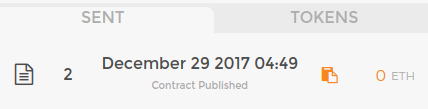
\includegraphics[width=10cm]{../pics/ethereum/metamask-contract-published}
	\end{figure}
	\vspace{-1em}
	\begin{enumerate}
		\item Select the ``Sent'' tab
		\item Check the orange Copy icon (Tx Hash) 
		\item Click on ``Contract Published''
		\item That should bring you to Etherscan (see next page)
	\end{enumerate}
}

\frame{
	\frametitle{Verify the status of your transaction on Etherscan}
	\begin{figure}
		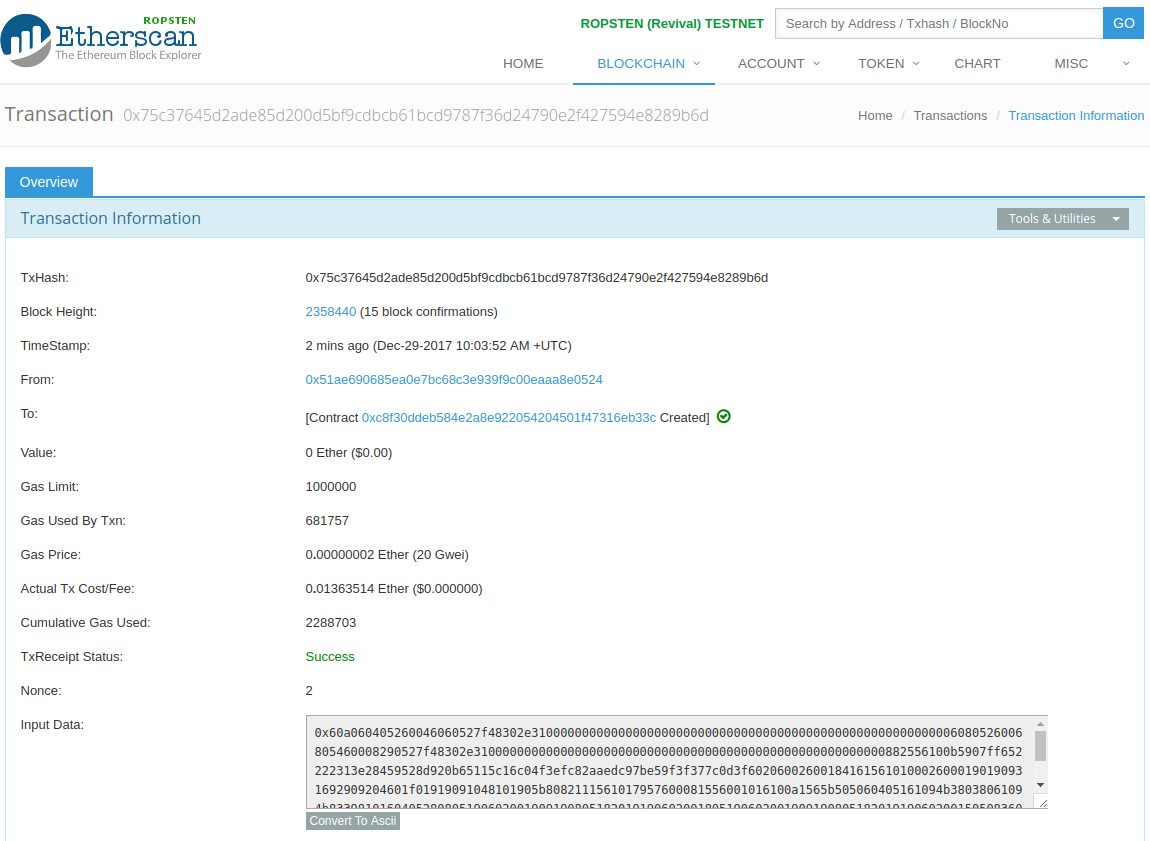
\includegraphics[width=10cm]{../pics/ethereum/etherscan-contract}
		\captionsetup{justification=centering}
		\caption*{Transaction Information: note the ``To'' line with your contract address}
	\end{figure}
}

\frame{
	\frametitle{Watch your Token}
	\begin{columns}
	\column{0.5\textwidth}
		\begin{figure}
			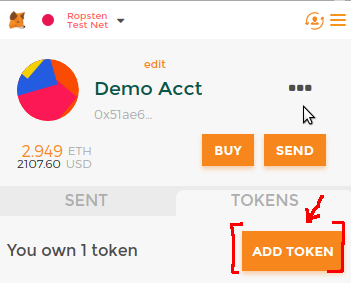
\includegraphics[width=3cm]{../pics/ethereum/metamask-add-token-1}
		\end{figure}
	\column{0.5\textwidth}
		\begin{figure}
			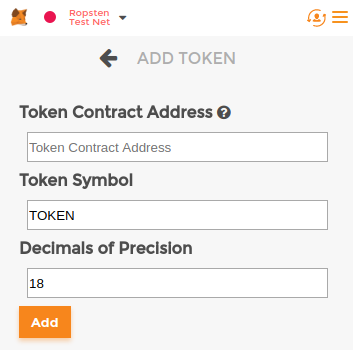
\includegraphics[width=3cm]{../pics/ethereum/metamask-add-token-2}
		\end{figure}
	\end{columns}
	\begin{enumerate}
		\item Click on the ``Add Token'' button
		\item Wait for the next window (picture on the right)
		\item Copy your contract address (from Etherscan)
		\item Go back to your Token Factory tab, which should show an UI to interact with your contract or go to the URL: https://tokenfactory.surge.sh/\#/token/0x... (replace 0x... by your contract address)
		\item Move coins around
		\item In MetaMask, click on your token to check the tx on Etherscan 
	\end{enumerate}
}

% ======================================================================================================
%                         Mint your own token (the programmatic way) 
% ======================================================================================================
\subsection{The programmatic way}

\frame{
	\frametitle{}
	\centering\Huge
	Too easy?\\
	\vspace{2em}
	Let's code it in Solidity\\like the pros!
}

\frame{
	\frametitle{Compile your first ERC-20 Smart Contract}
	\begin{figure}
		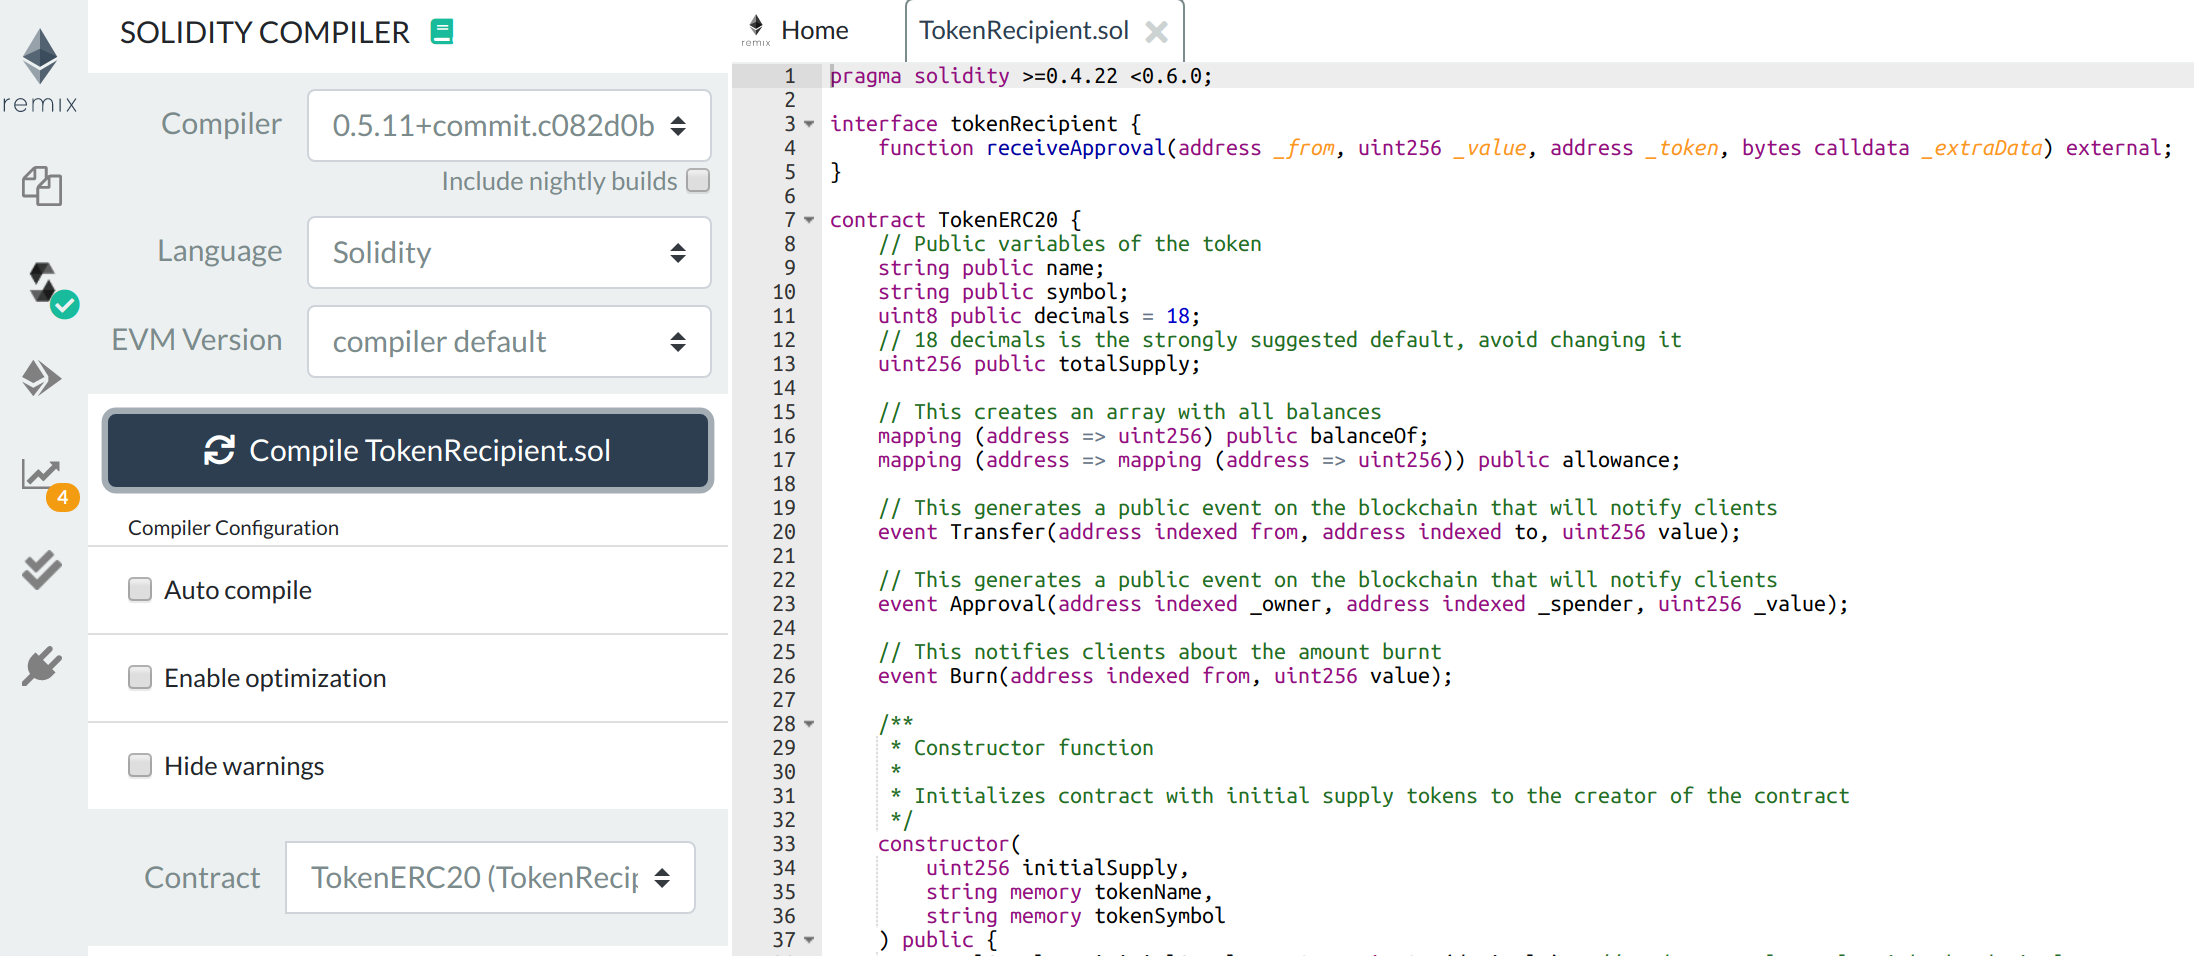
\includegraphics[width=10cm]{../pics/ethereum/remix-token-sol-compiled}
	\end{figure}
	\begin{enumerate}
		\item Open the Remix IDE at \url{http://remix.ethereum.org}
		\item Close the ballot file 
		\item Create a new file named TokenRecipient.sol 
		\item Copy the code from \url{https://raw.githubusercontent.com/ethereum/ethereum-org/master/solidity/token-erc20.sol}
		\item Your compiler can be the default one (5.11)
		\item Click the "Compile TokenRecipient.sol" button
	\end{enumerate}
%	Reference:\\
%	\href{https://github.com/ethereum/EIPs/blob/master/EIPS/eip-20-token-standard.md}{ERC-20 Token Standard}
}

\frame{
	\frametitle{Deploy your smart contract}
	\begin{figure}
		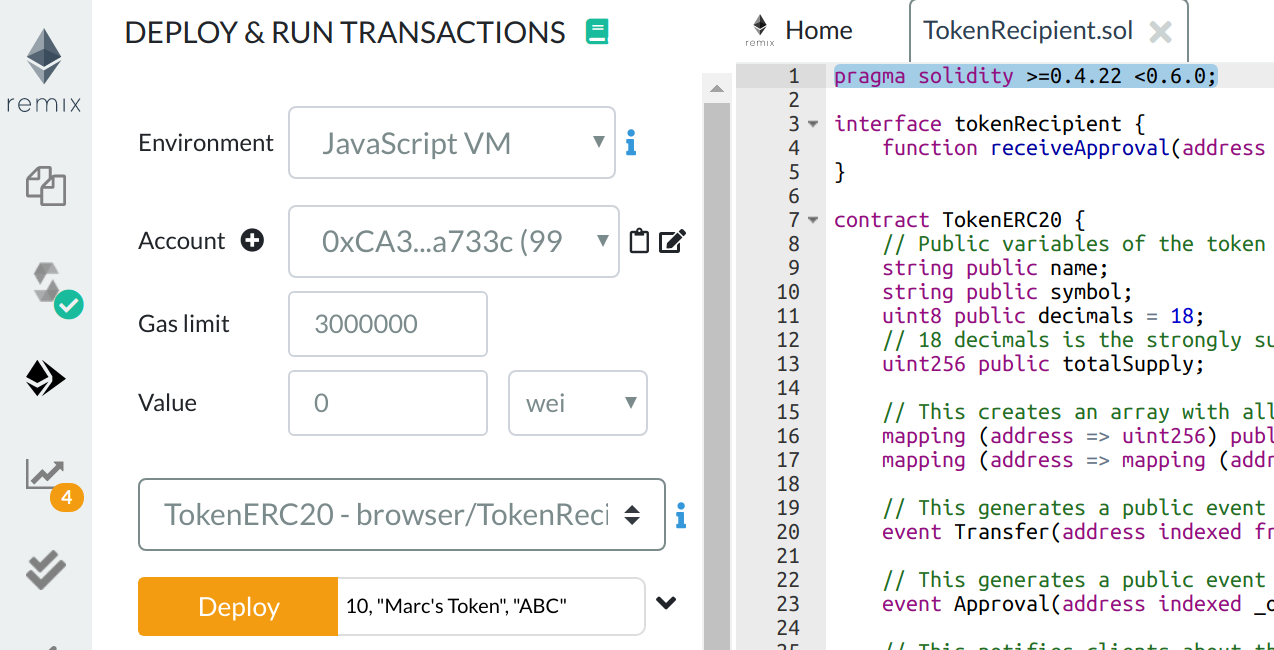
\includegraphics[width=10cm]{../pics/ethereum/remix-token-to-deploy-filled}
	\end{figure}
	\begin{enumerate}
		\item Go to the "Deploy and run transaction screen (Ethereum-like logo on the left bar) 
		\item Fill in the parameters next to the orange "Deploy" button
		\item Click the "Deploy" button
	\end{enumerate}
}

\frame{
	\frametitle{Deployed Contract}
	\begin{figure}
		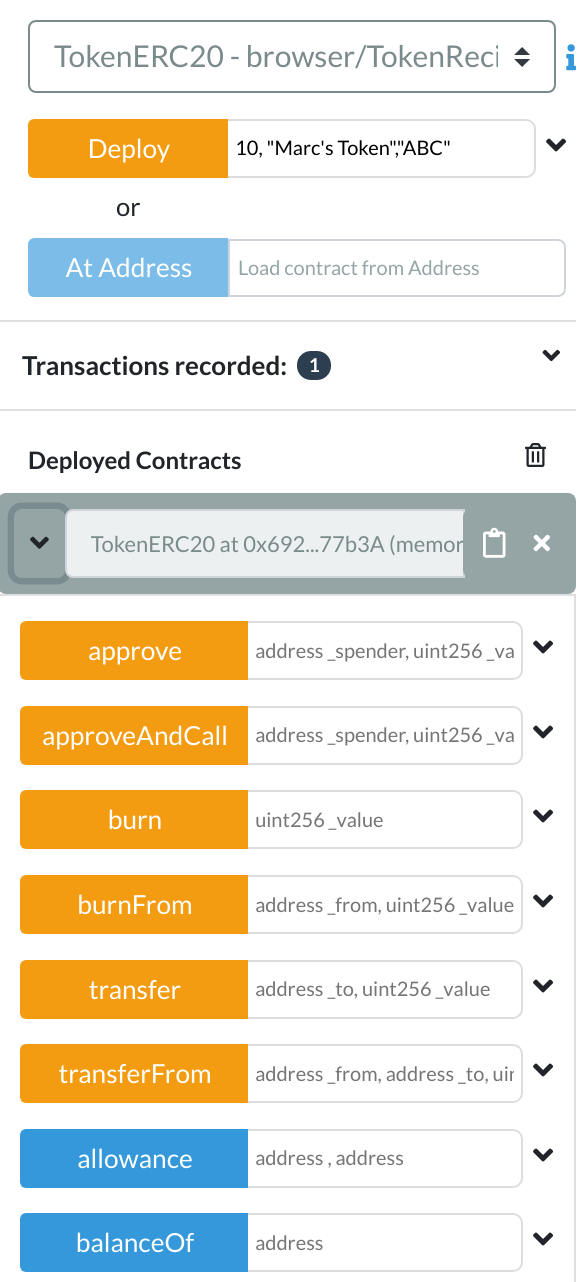
\includegraphics[height=6cm]{../pics/ethereum/remix-contract-deployed}
	\end{figure}
	\begin{enumerate}
		\item Expand the "Deployed Contracts"
		\item All the contract functions are available from Remix
	\end{enumerate}
}


% ======================================================================================================
%                         Ethereum 
% ======================================================================================================
\section{Introduction to Ethereum}
\frame{
	\frametitle{Ethereum}
	%\framesubtitle{}
	\begin{columns}
	\column{0.5\textwidth}
		Ethereum is a \textbf{decentralized platform that runs smart contracts}: applications that run exactly as programmed without any possibility of downtime, censorship, fraud or third party interference.\\
		--- \url{https://ethereum.org}
	\column{0.5\textwidth}
		\begin{figure}
			
\includegraphics[height=6cm]{../pics/ethereum/471px-Ethereum_logo_2014}
		\end{figure}
	\end{columns}
}

\frame{
	\frametitle{A short history of Ethereum}
	Key Milestones:
	\begin{itemize}
		\item (late 2013) Vitalik Buterin describes Ethereum in a paper
		\pause
		\item (Summer 2014) Ethereum raises more than \$14 million in pre-sale
		\pause
		\item (July 30, 2015) Launch of Frontier, initial (beta) version of Ethereum 
		\pause
		\item (March 14, 2016) Launch of Homestead, first production release
		\pause
		\item (Spring 2016) The DAO
		\pause
		\item (July 2, 2016) ETH -- ETC split
		\pause
		\item (October 16, 2017) Launch of Metropolis (vByzantium) --version 3
		\pause
		\item (2017) ETH goes from ~\$7 to more than \$700 (100x increase)
	\end{itemize}
	\vspace{1em}
	\emph{Check the \href{https://cdn4.benzinga.com/files/images/2017/July/05/invezz-eth-history-base.jpg}{nice infographic (\cite{ethinfographic})}.}\\
	\vspace{.5em}
	Also, see the official \href{https://github.com/ethereum/wiki/wiki/White-Paper}{\emph{Ethereum White Paper}}.
}

%\frame{
%	\frametitle{Store of value}
%	\begin{figure}
%	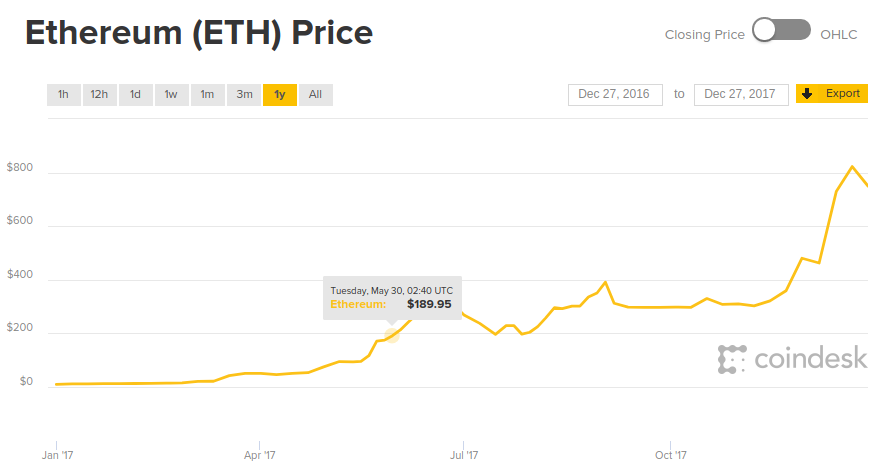
\includegraphics[height=6cm]{../pics/ethereum/ETH-price-2017}
%		\caption{ETH price (\cite{coindesk:eth-price})}
%		%\caption{Credit: \href{https://www.coindesk.com/ethereum-price/}{Coindesk}}
%	\end{figure}
%}

\frame{
	\frametitle{Decentralization}
	\begin{figure}
		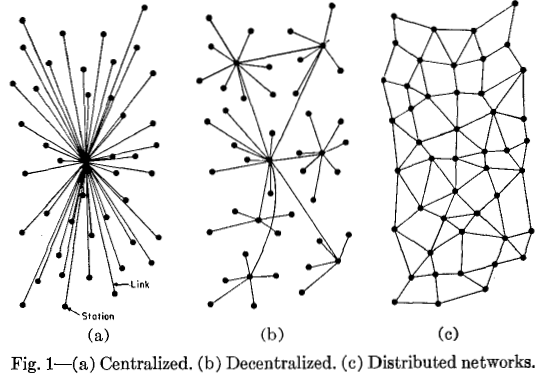
\includegraphics[height=6cm]{../pics/ethereum/networktypes}
	\end{figure}
}

\frame{
	\frametitle{Client Types}
	\begin{itemize}
		\item Full node 
		\pause
		\item Light node 
		\pause
		\item Something in between (e.g. ``fast'' for geth)
	\end{itemize}
}

\frame{
	\frametitle{Disk Space}
	\framesubtitle{Full Archive Ethereum node}
	\begin{figure}
	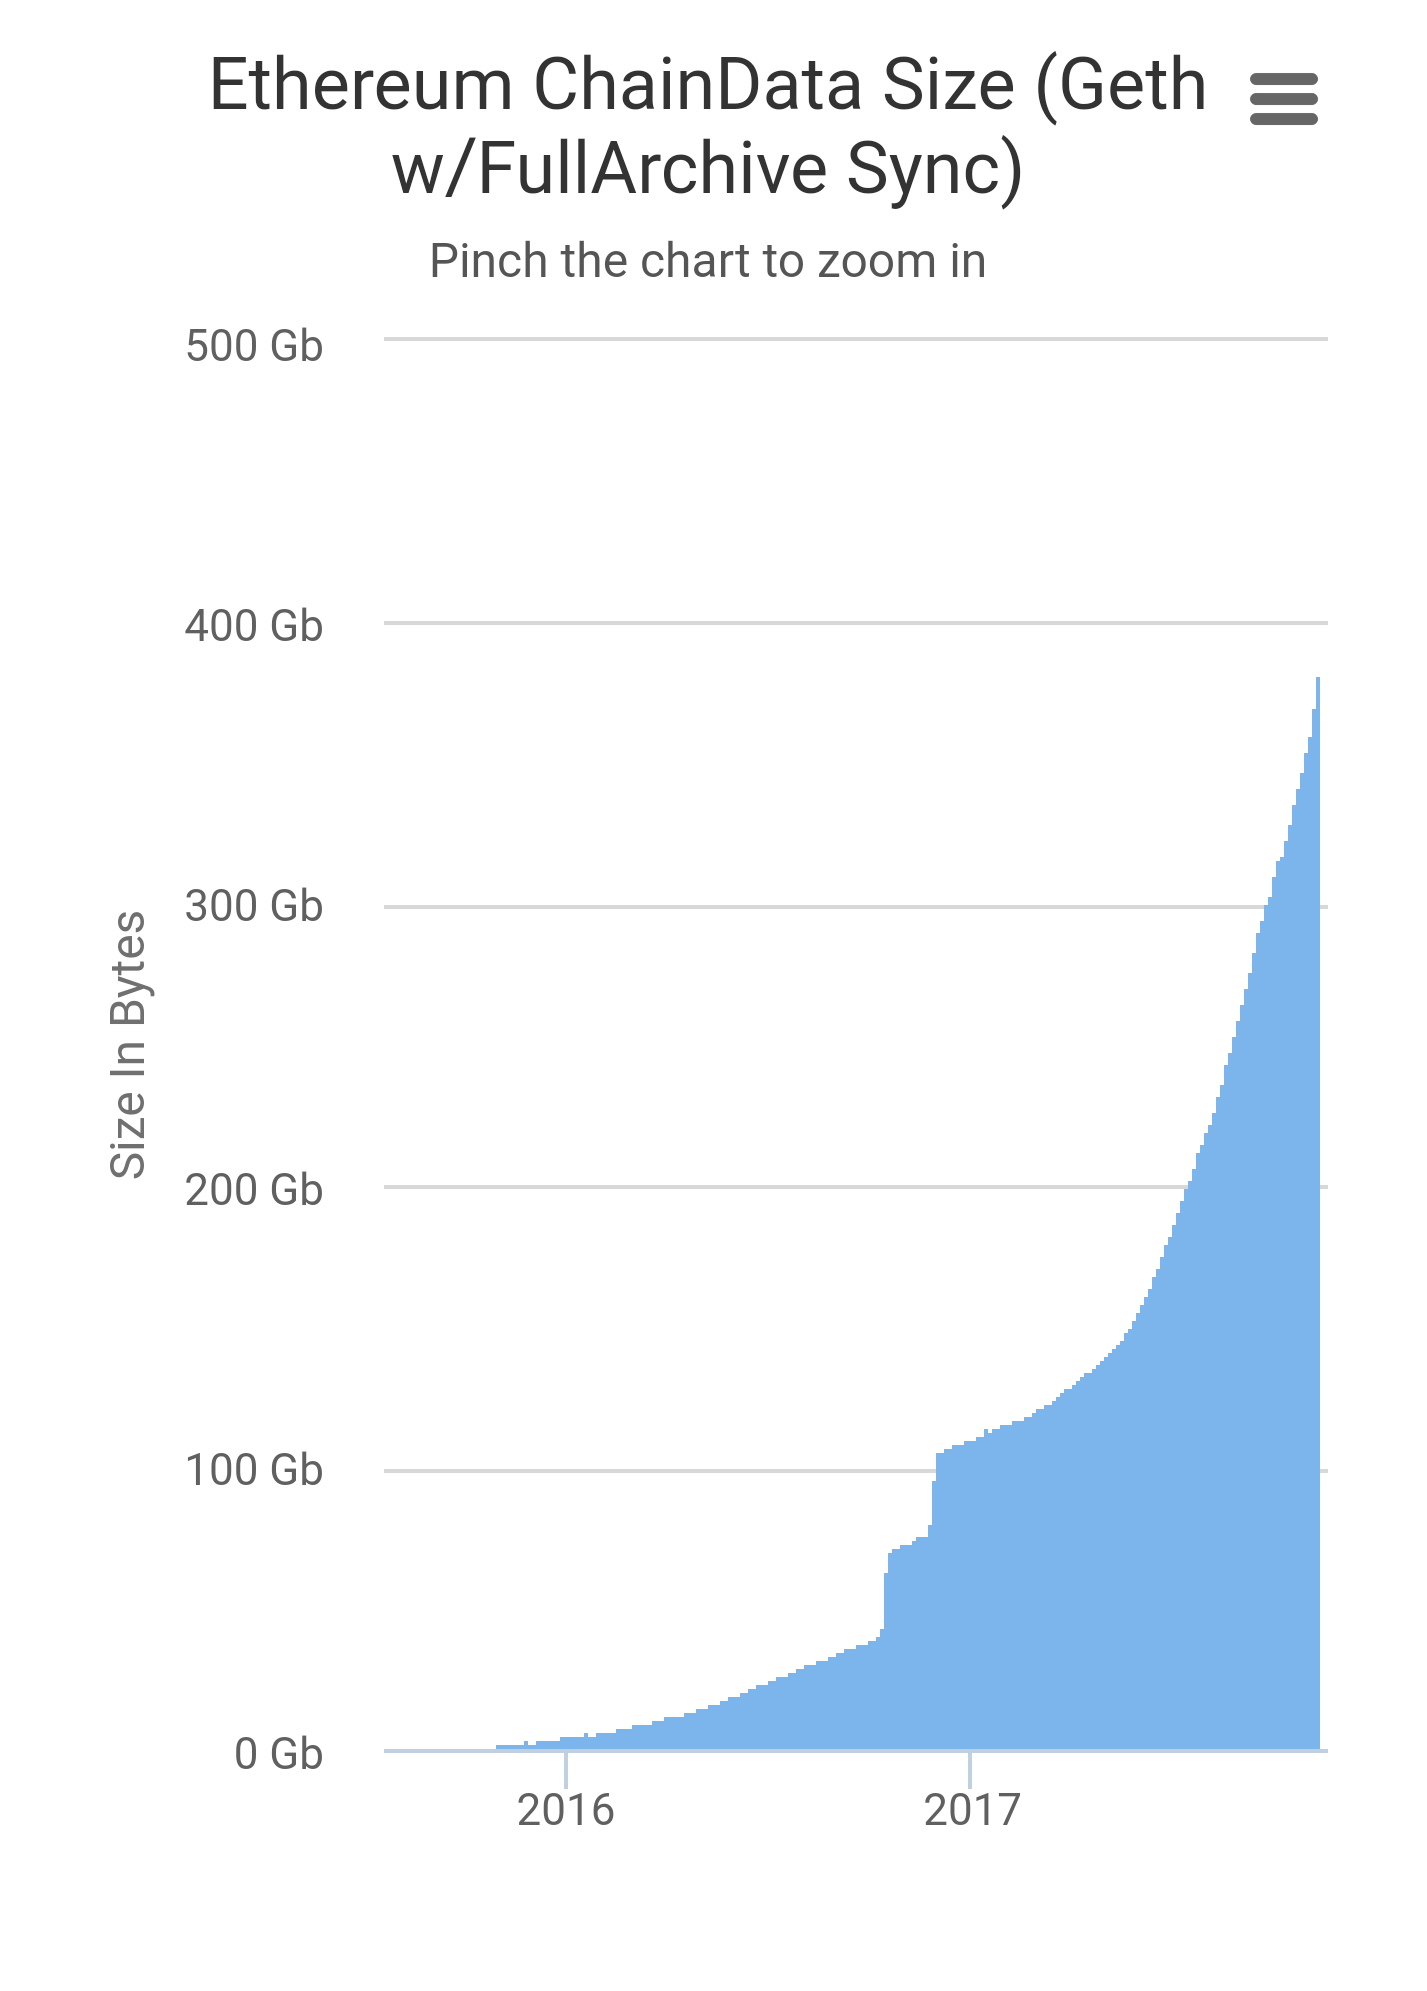
\includegraphics[height=6cm]{../pics/ethereum/geth-full-archive}
		\caption{Miners need a lot of space (\cite{reddit:chaindatasize})}
	\end{figure}
}

\frame{
	\frametitle{Practical Applications}
	\framesubtitle{for personal or business use}
	\begin{figure}
	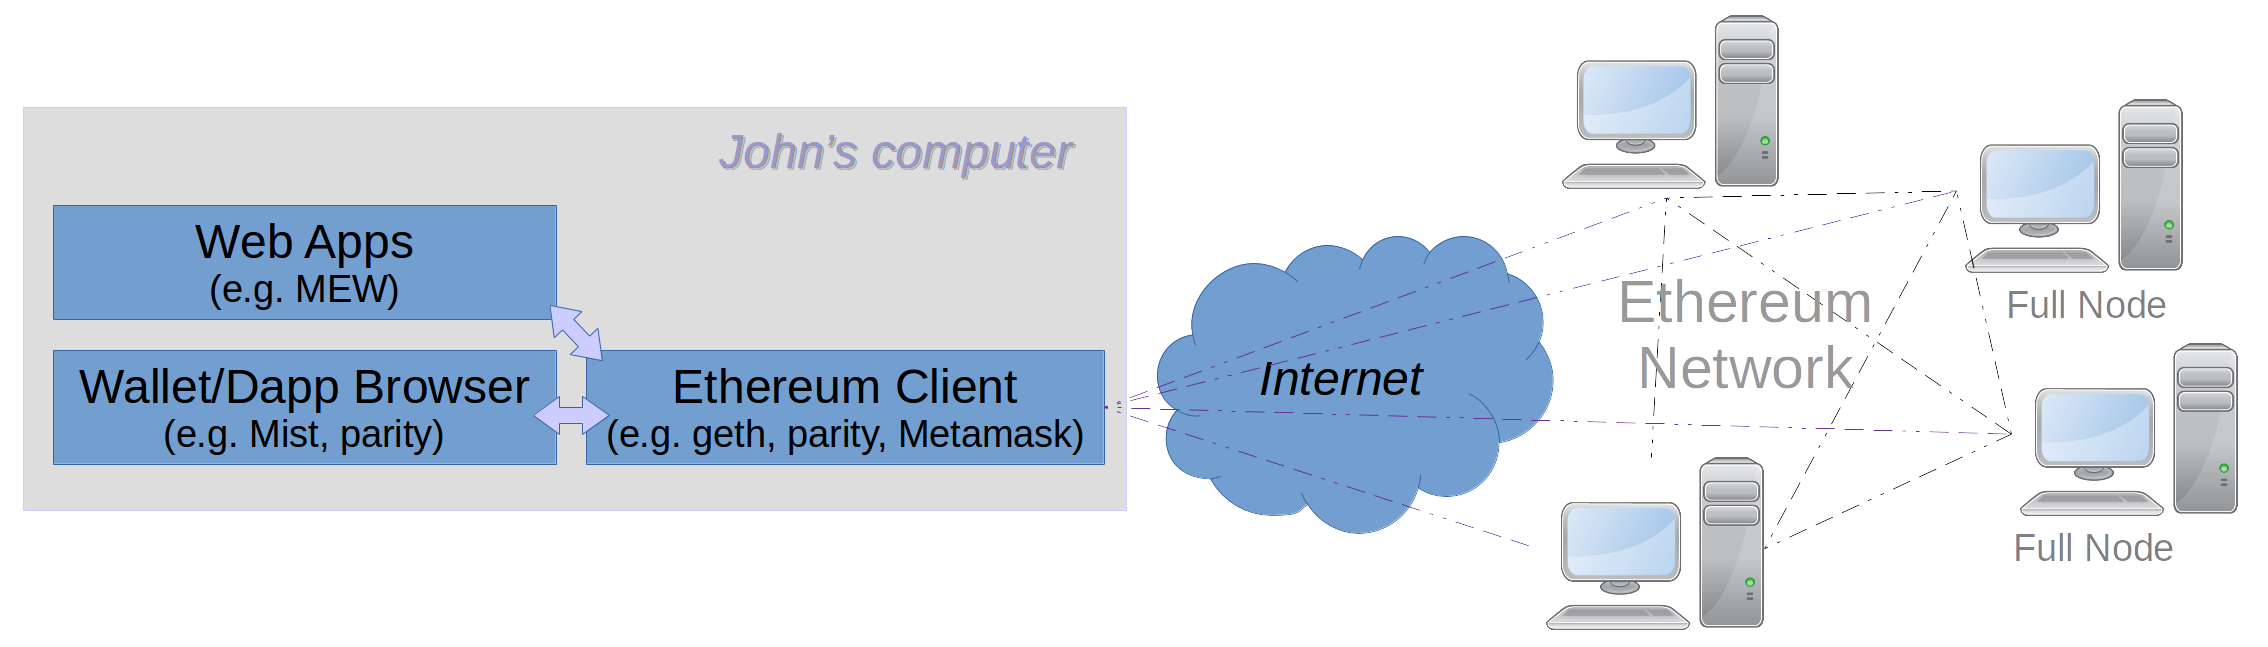
\includegraphics[width=12cm]{../pics/ethereum/ethereum-dapp-arch}
	\end{figure}
}

\frame{
	\frametitle{Reference books}
	\framesubtitle{Blockchain applications}
	\begin{columns}[T]
	\column{0.5\textwidth}
		\begin{figure}
			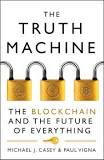
\includegraphics[height=4cm]{../pics/books/book-casey-truth.jpeg}
			\captionsetup{justification=centering}
			\caption{Book from \cite{casey2018:truth}}
		\end{figure}
	\column{0.5\textwidth}
		\begin{figure}
			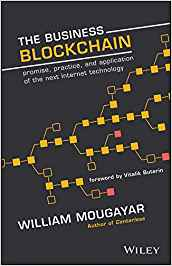
\includegraphics[height=4cm]{../pics/books/book-mougayar-business}
			\captionsetup{justification=centering}
			\caption{Book from \cite{mougayar:business}}
		\end{figure}
	\end{columns}
}

\frame{
	\frametitle{Reference books}
	\framesubtitle{More recent publications}
	\begin{columns}[T]
	\column{0.5\textwidth}
		\begin{figure}
			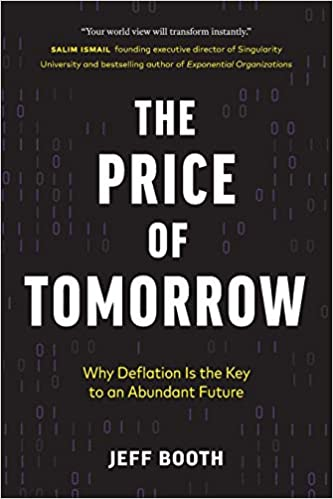
\includegraphics[height=4cm]{../pics/books/booth-pricetomorrow}
			\captionsetup{justification=centering}
			\caption{Book from \cite{Booth_Jeff2020-01-14}}
		\end{figure}
	\column{0.5\textwidth}
		\begin{figure}
			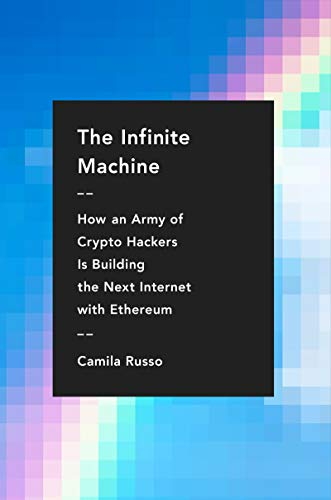
\includegraphics[height=4cm]{../pics/books/russo-infinitemachine}
			\captionsetup{justification=centering}
			\caption{Book from \cite{Russo_Camila2020-07-14}}
		\end{figure}
	\end{columns}
}

\frame{
	\frametitle{Ultimate references}
	The must-read white paper from legendary Satoshi Nakamoto: \textit{Bitcoin: A Peer-to-Peer Electronic Cash System} (\citeyear{satoshi:bitcoin-paper}),\\
	\vspace{1em}
	the Ethereum white paper from home-town Toronto Vitalik Buterin: \textit{A Next-Generation Smart Contract and Decentralized Application Platform} (\citeyear{buterin:ethereum-paper}),\\
	\vspace{1em}
	and the yellow paper authored by Prof. Gavin Wood: \textit{Ethereum: A secure decentralised generalised transaction ledger} (\citeyear{wood:ethereum-yellow-paper}).
}


%\frame{
%	\frametitle{}
%}



